%==============================================================================
\chapter{In silico identification of potential calcium dynamics and sarcomere targets for recovering left ventricular function in rat heart failure with preserved ejection fraction}\label{cha:chapter7}
%==============================================================================
%
%
%
\begin{remark}{Outline}
    In this chapter, we build an emulator that can map both calcium dynamics, sarcomere, tissue and haemodynamics properties to the LV function, using the personalised SHAM rat heart contraction model as simulator (Section~\ref{sec:ch7training_dataset_emulators_global_sensitivity_analysis}). After having characterised the model outputs' global sensitivities to model inputs (Section~\ref{sec:ch7model_emulators_and_output_sensitivities}), starting from the healthy reference rat model we create a model of the $20$-week old obese ZSF1 rat, a well-established animal model of HFpEF (Section~\ref{sec:ch7building_a_model_of_the_20_week_old_obese_zsf1_rat}). We then use different sub-groups of input parameters as targets of a re-fitting, history matching procedure, with the aim of recovering the ZSF1 rat model back to the healthy state (Section~\ref{sec:ch7in_silico_recovering_the_zsf1_rat_towards_healthy_conditions}). The selected groups of parameters mimic the action of possible calcium-, thin filament-, thick filament-, whole sarcomere-targeting compounds. We show that using the implemented framework it is possible to \textit{in silico} efficiently identify possible pharmacological interventions on the sarcomere to treat HFpEF in rats (Section~\ref{sec:ch7recovered_lv_function_in_zsf1_rats}). We then provide a discussion and address specific limitations (Section~\ref{sec:ch7discussion}), and we conclude with a brief summary (Section~\ref{sec:ch7summary}).
\end{remark}


%
%
%
\section{Motivation}\label{sec:ch7motivation}
Heart failure (HF) is a progressive and prevalent disease. Approximately $\SI{50}{\percent}$ of patients have heart failure with preserved ejection fraction (HFpEF), characterised by impaired myocardial relaxation and often secondary to hypertension and obesity. There are limited evidence-based pharmacotherapies for HFpEF and thus HFpEF represents an unmet clinical need. Patients currently receive either angiotensin-converting enzyme inhibitors/aldosterone receptor blockers, $\Ca$ channel blockers or beta-blockers, but the mortality and the morbidity associated with the disease have so far remained high~\cite{Adamczak:2020}.

\vspace{0.2cm}
Animal models constitute a valuable research tools to investigate HFpEF, as co-morbidities and other confounding factors can be more precisely controlled than in the clinical setting. However, there are no perfect animal models for HFpEF, and this is in part because it is difficult to fulfil all the features observed in human disease at the same time in animals. The currently available animal models of HFpEF have attempted to reproduce the dominant factors typically documented to cause diastolic dysfunction and HFpEF. They fall across the following macro-categories: aortic banding and systemic hypertension, diabetes mellitus and obesity, cardiometabolic syndrome and ageing. All of these animal models have been successfully established in rodents~\cite{Conceicao:2016}. Regardless of the animal model used in the process of drug discovery and development at preclinical stages, identifying pharmacological interventions that recover physiological function in the HFpEF diseased animal still remains a challenge.

\vspace{0.2cm}
In this study we aim to predict changes in myocyte function that recovers whole heart function. First, we propose a multi-scale mathematical model that maps ion channel and sarcomere function through to whole organ pump function in a HFpEF rat heart. Specifically, we want to build an \textit{in silico} representation of the \textit{20-week old obese ZSF1 rat}, a recently proposed HFpEF animal model. This model can then be used to identify cellular function that can be manipulated to recovered whole heart function. We propose to use this animal model to provide indication of pharmacological targets by simulating and testing their different mechanisms of action. The $20$-week old obese ZSF1 rat presents many features of a cardiometabolic syndrome such as hypertension, obesity, type $2$ mellitus, insulin resistance and HF, developing a diastolic dysfunction in parallel with left ventricular (LV) hypertrophy and left atrial dilation. As this animal model also presents exercise intolerance, an important feature diagnosed in humans, it currently constitutes a well-established~\cite{Conceicao:2016} animal model of HFpEF. From now on, we will refer to the ``$20$-weeks old obese ZSF1 rat" as the ``ZSF1 rat" for brevity.


%
%
%
\section{Rat data}\label{sec:ch7raddata}
In order to create a mathematical model of the ZSF1 rat, we first needed to characterise its LV systolic and diastolic functions. For this purpose, we performed a literature search on PubMed (date 09/03/2021) with query: ``(rat) AND (ZSF1) AND (haemodynamic)". The search gave $32$ results and we analysed them all. Of these, $19$ contained information about LV haemodynamic measurements. All the $19$ studies~\cite{Abdellatif:2016, Bowen:2017, Bowen:2018, Brandt:2019, Cuijpers:2020, Davila:2019, Hamdani:2013, Hohendanner:2018, Lai:2016, Leite:2015, Leite:2015*a, Leite:2019, Nguyen:2020, Park:2020, Salah:2018, Schmederer:2018, Stolina:2020, Van-Dijk:2016, Wang:2020} had been conducted on male rats at the age of $20$ weeks, and diastolic dysfunction was confirmed by echocardiographic measurements (decreased E/A, increased E/E', increased LA area). We identified common phenotypes in these obese ZSF1 rats' haemodynamics compared to their respective control (lean ZSF1 rat) as described by $4$ LV features, namely $\textrm{EF}$ (no change), $\textrm{PeakP}$ (increased), $\textrm{maxdP}$ (increased), $\textrm{Tau}$ (increased). To regularise observed changes in ZSF1 rats from multiple labs, we considered the average percentage changes between ZSF1 rats and local control animals. These are summarised in Table~\ref{tab:obesezsf1data}.

\begin{table}[ht!]
    \myfloatalign
    \begin{tabularx}{\textwidth}{lXX}
    \toprule
    \tableheadline{LV feature}                  & \tableheadline{Exp. variability ($\SI{}{\percent}$)} & \tableheadline{Reference} \\
    \midrule
    $\textrm{EF}$    & $103.95\pm 7.62$  & \cite{Bowen:2017, Cuijpers:2020, Hamdani:2013, Leite:2015, Leite:2019, Salah:2018, Stolina:2020, Leite:2015*a, Schmederer:2018} \\
    $\textrm{PeakP}^{*}$ & $119.26\pm 6.07$  & \cite{Leite:2015, Leite:2019} \\
    $\textrm{maxdP}^{*}$ & $125.46\pm 5.26$  & \cite{Bowen:2017, Hamdani:2013, Leite:2015, Leite:2015*a, Schmederer:2018} \\
    $\textrm{Tau}^{*}$ & $141.97\pm 13.67$ & \cite{Bowen:2017, Cuijpers:2020, Hamdani:2013, Leite:2015, Leite:2019, Salah:2018, Stolina:2020} \\
    \bottomrule
    \end{tabularx}
    \caption{Experimental ZSF1 obese rat haemodynamic data. For each LV feature of interest, mean and standard deviation values are given as percentages of the related control mean values. Asterisked $(\cdot)^*$ features' changes were reported to be statistically significant.}
    \label{tab:obesezsf1data}
\end{table}



%
%
%
\section{Methods}\label{sec:ch7methods}


%
%
%
\subsection{Rat heart contraction model}\label{sec:ch7rat_heart_contraction_model}
We modelled the healthy rat heart using the personalised SHAM rat heart contraction model derived in Section~\ref{sec:ch4fittedmodels}. This rat model will be referred to as ``SHAM" throughout the next sections. Again, this model (or simulator) can be seen as a multi-scale map from input parameters to output features.

% We selected specific parameters as representative regulators of each of these sub-models, for a total of $16$ parameters. The calcium transient represented the end output of the cellular electrophysiology model used for the sarcomere contraction model, and was simulated only once at this stage. This is because the first $4$ parameters we selected for the multi-scale map input encoded the whole shape of the calcium transient and could independently scale its main properties (diastolic concentration, amplitude, time to peak and recovery time, see~\nameref{S1_Text} for more details). Of the other selected parameters, $8$ described the sarcomere dynamics ($4$ parameters were thin filament-related and $4$ were thick filament-related), and $4$ parameters described boundary conditions and tissue properties. The $16$ parameters considered are defined in Table~\ref{tab:paramswithdef}. 

\vspace{0.2cm}
We augmented the list of parameters used previously (Sections~\ref{sec:ch4ratheartcontractionmodel}--\ref{sec:ch5ratheartcontractionmodel}) in order to have a more comprehensive description of both the calcium and sarcomere dynamics, tissue and haemodynamic boundary conditions' properties, by considering a total of $16$ parameters. Specifically, $4$ parameters encoded the shape of the $\Ca$ transient (Section~\ref{sec:ch6encoding_ca_transient_variations}), $8$ parameters described the sarcomere dynamics ($4$ parameters were thin filament-related and $4$ were thick filament-related), and $4$ parameters described tissue and boundary conditions' properties. The full list of parameters considered is reported in Table~\ref{tab:paramswithdeffinal}.

\begin{table}[ht!]
    \myfloatalign
    \begin{tabularx}{\textwidth}{llX}
    \toprule
    \tableheadline{Parameter} & \tableheadline{Units}                   & \tableheadline{Definition} \\
    \midrule
    $\dca$                    & $\SI{}{\micro\Molar}$                   & diastolic $\Ca$ concentration \\
    $\ampl$                   & $\SI{}{\micro\Molar}$                   & $\Ca$ concentration signal amplitude \\
    $\tp$                     & $\SI{}{\milli\second}$                  & time to peak $\Ca$ concentration \\
    $\rtf$                    & $\SI{}{\milli\second}$                  & time to half-maximal relaxation from peak $\Ca$ concentration \\
    $\Caif$                   & $\SI{}{\micro\Molar}$ & reference $\Ca$ thin filament sensitivity \\
    $\betaone$                & $-$                                     & phenomenological tension length-dependence scaling factor \\
    $\koff$                   & $\SI{}{\per\milli\second}$              & unbinding rate of $\Ca$ from TnC \\
    $\ntrpn$                  & $-$                                     & $\Ca$-TnC binding degree of cooperativity \\
    $\kxb$                    & $\SI{}{\per\milli\second}$              & cross-bridges cycling rate \\
    $\nxb$                    & $-$                                     & cross-bridge formation degree of cooperativity \\
    $\trpnf$                  & $-$                                     & fraction of $\Ca$-TnC bounds for half-maximal cross-bridges activation \\
    $\tref$                   & $\SI{}{\kilo\pascal}$                   & maximal reference tension \\
    $\p$                      & $\SI{}{\kilo\pascal}$                   & end-diastolic pressure \\
    $\pao$                    & $\SI{}{\kilo\pascal}$                   & aortic systolic pressure \\
    $\Z$                      & $\SI{}{\mmHg\second\per\milli\liter}$   & aortic characteristic impedance \\
    $\Cone$                   & $\SI{}{kPa}$                            & tissue stiffness \\
    \bottomrule
    \end{tabularx}
    \caption{Model parameters and their definitions.}
    \label{tab:paramswithdeffinal}
\end{table}

\vspace{0.2cm}
As for the simulator output, we characterised the LV function using the same $12$ scalar features used in the previous analysis (Table~\ref{tab:lvfeatures}) with the addition of other $2$ features (Table~\ref{tab:lvfeaturesfinal}), for a total of $14$ features.

\begin{table}[ht!]
    \myfloatalign
    \begin{tabularx}{\textwidth}{llX}
    \toprule
    \tableheadline{LV feature}                  & \tableheadline{Units}                         & \tableheadline{Definition} \\ \midrule
    $\textrm{SV}$                   & $\SI{}{\micro\liter}$                  &  stroke volume \\
    $\textrm{Tau}$   & $\SI{}{\milli\second}$ & isovolumetric pressure relaxation time constant \\
    \bottomrule
    \end{tabularx}
    \caption{Indexes of LV systolic and diastolic functions.}
    \label{tab:lvfeaturesfinal}
\end{table}

\vspace{0.2cm}
The obtained simulator map had thus the following form:
%
\begin{align}\label{eq:fsimulfinal}
    f_{simul}\colon\mathbb{R}^{16} &\to\underbrace{\mathbb{R}\times\cdots\times\mathbb{R}}_{14\,\text{times}} \\
    \mathbf{x} &\mapsto (y_1,\,\dots,\,y_{14}) \nonumber
\end{align}

\vspace{0.2cm}\noindent
When running the simulator at a new parameter point, as we were using the personalised SHAM rat model, all the other parameters were kept fixed to its reference parameter values (Table~\ref{tab:shamabbestfitparamvalues}) when applicable, or to the Land et al.~\cite{Land:2012} model baseline values when otherwise.

\vspace{0.2cm}
To reduce computational costs, we will again train low cost emulators to be a surrogate for the full model. This will allow to map input parameters to output LV features both in a deterministic (using the simulator) and in a probabilistic (using the emulator) way, as shown in Figure~\ref{fig:multiscalemap}.

\begin{figure}[ht!]
    \myfloatalign
    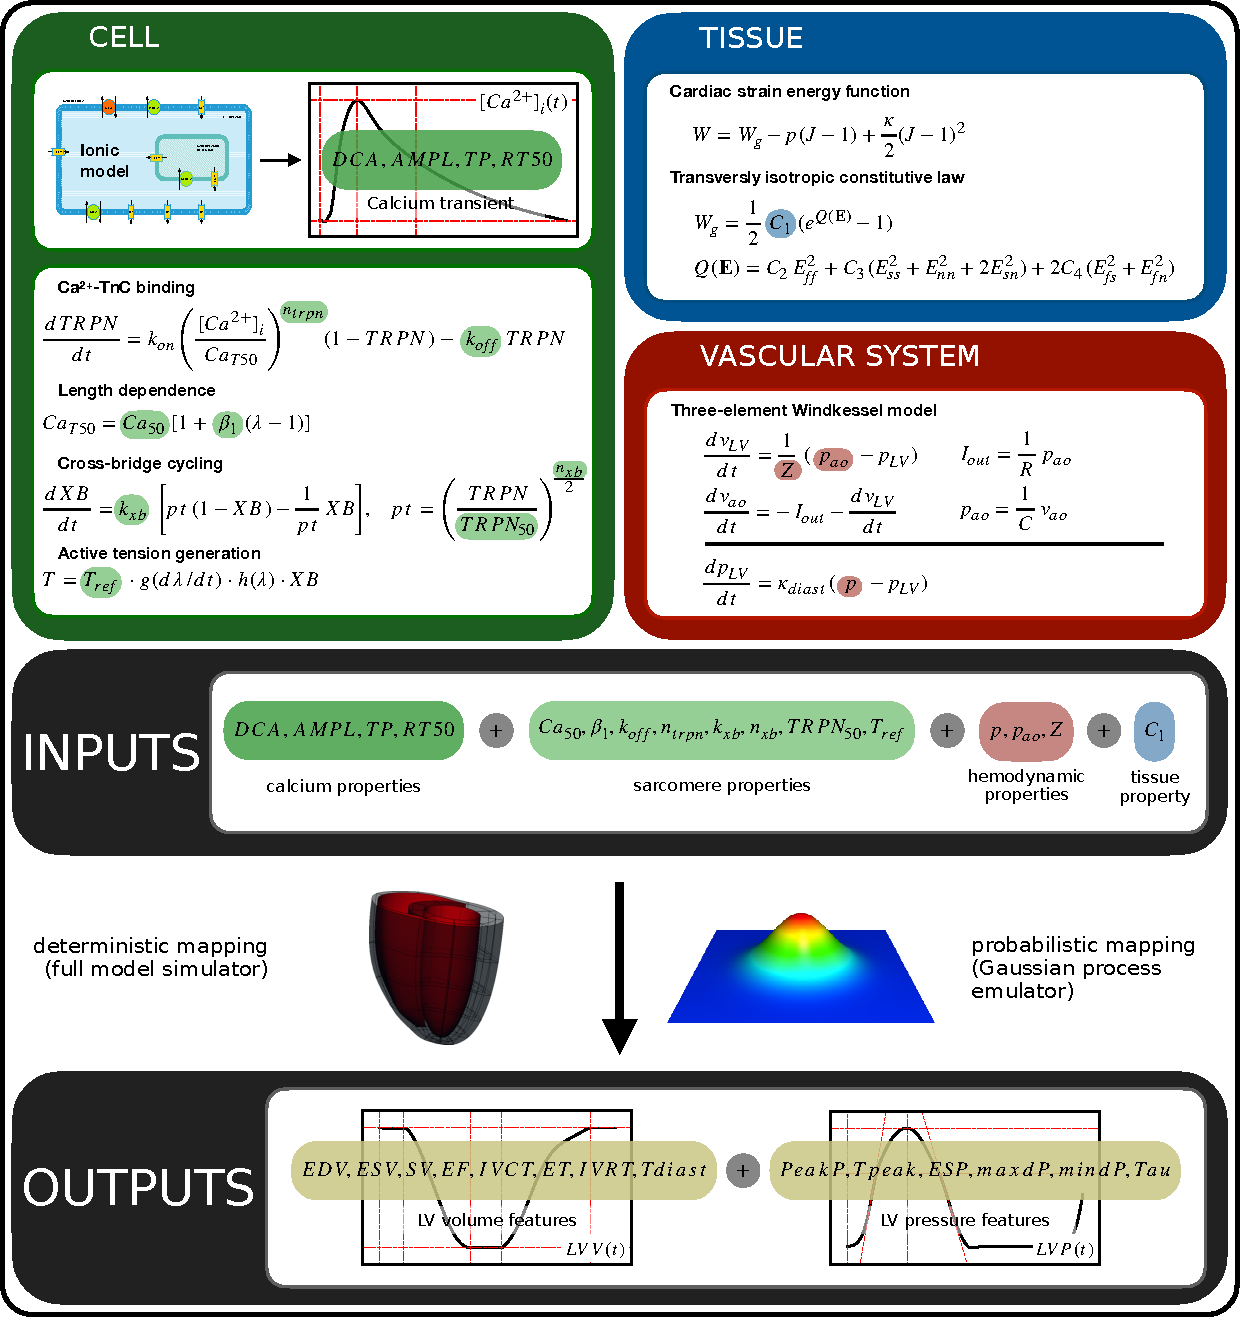
\includegraphics[width=\textwidth]{figures/chapter07/Fig_1.pdf}
    \caption{$\mathbf{3}$D biventricular rat heart contraction model multi-scale map. Chosen $16$ input parameters are calcium transient and sarcomere properties (green), haemodynamics properties (red) and tissue properties (blue). The output features of interest are $14$ indexes (yellow) characterising the LV function and are extracted from the LV pressure and volume curves. The input parameters (Table~\ref{tab:paramswithdeffinal}) can be quantitatively be mapped to the output features (Tables~\ref{tab:lvfeatures}--\ref{tab:lvfeaturesfinal}) either by running the full model or by making predictions using trained GPEs.}
    \label{fig:multiscalemap}
\end{figure}


%
%
%
\subsection{Input parameter space}\label{sec:ch7inputparameterspace}
The input parameter space $X\subset\mathbb{R}^{16}$ of the simulator map $f_{simul}$ introduced in equation~\eqref{eq:fsimulfinal} was defined as the hypercube obtained by the Cartesian product of $16$ one-dimensional parameter ranges. Each parameter interval was constructed with lower and upper bounds given as percentages of the SHAM rat heart model reference parameter values (Table~\ref{tab:shamabbestfitparamvalues}), based on a literature search and preliminary sensitivity analysis studies.

\vspace{0.2cm}
Specifically, for the $\Ca$ transient parameters/features ($\ampl$, $\dca$, $\tp$ and $\rtf$) we performed a literature search to understand how these values could change when going from diseased to control animal in rat HF. We collected experimental observations from $30$ experimental studies~\cite{Abdellatif:2021, An:2019, Berni:2009, Bode:2020, Bode:2021, Call:1998, Chang:1997, Chen:2020, Curl:2018, Deel:2017, Gattoni:2017, Hohendanner:2018, Hu:2011, Ito:1997, Kagaya:1995, Kagaya:1996, Kennedy:2003, Kilfoil:2020, Kim:2017, Loennechen:2002, Loennechen:2002*a, Lyon:2009, Lyon:2011, Maczewski:2008, Maier:1998, Meissner:1998, Min:2002, Miranda-Silva:2020, Rouhana:2019, Sadredini:2016} on both HFrEF and HFpEF animal models, including AB (aortic-banded rat), TAC (transverse aortic constricted rat), CHF (rat with chronic heart failure), MI (rat with myocardial infarction), ZSF1 (Zucker diabetic fatty rat) DSS (Dhal salt-sensitive rat). To normalise observations across studies with different animal models and different pacing frequencies used for $\Ca$ transients' recording ($0.5$, $0.333$, $1$, $3$, $4$, $6$, $\SI{7}{\hertz}$), we averaged mean percentage variations from control to diseased animals for each of the four $\Ca$ transient parameters. Minimum and maximum percentage variations observed experimentally are reported as ranges in Table~\ref{tab:calitranges}.

\begin{table}[ht!]
    \myfloatalign
    \begin{tabularx}{\textwidth}{llX}
    \toprule
    \tableheadline{Parameter} & \tableheadline{Exp. variability ($\SI{}{\percent}$)} & \tableheadline{Reference} \\
    \midrule
    $\dca$                    & $[38.00,\,200.0]$ & \cite{Abdellatif:2021, An:2019, Berni:2009, Bode:2020, Bode:2021, Call:1998, Chang:1997, Chen:2020, Curl:2018, Deel:2017, Gattoni:2017, Hohendanner:2018, Hu:2011, Ito:1997, Kagaya:1995, Kagaya:1996, Kennedy:2003, Kilfoil:2020, Kim:2017, Loennechen:2002, Loennechen:2002*a, Lyon:2009, Lyon:2011, Maczewski:2008, Maier:1998, Meissner:1998, Min:2002, Miranda-Silva:2020, Rouhana:2019, Sadredini:2016} \\
    $\ampl$                   & $[30.41,\,203.23]$ & same as above \\
    $\tp$                     & $[100.00,\,151.26]$ & same as above \\
    $\rtf$                    & $[59.56,\,176.27]$ & same as above \\
    \bottomrule
    \end{tabularx}
    \caption{Calcium transient parameters' experimental variability in heart failure rat models.}
    \label{tab:calitranges}
\end{table}

\vspace{0.2cm}\noindent
The adopted range for the $\Ca$ transient parameters was $[\SI{10}{\percent},\,\SI{200}{\percent}]$ of the respective control values, which achieved a full coverage of the experimentally observed variability (Table~\ref{tab:calitranges}) while being nearly symmetric around the baseline value ($\SI{100}{\percent}$). The range for $\rtf$ parameter was further adjusted to $[\SI{10}{\percent},\,\SI{110}{\percent}]$ in order to limit the generation of implausible $\Ca$ transients (where the sum of the time to peak and the relaxation time exceed the cycle length) when randomly scaling the reference $\Ca$ transient (Algorithm~\ref{alg:caalg}, Section~\ref{sec:ch6encoding_ca_transient_variations}). Although the upper bound of this range seems not to cover the experimental observations fully, it is important to note that most heart failure studies are performed at non-physiological pacing rates ($\SI{0.3}{}$-$\SI{1}{\hertz}$), which allow much longer relaxation times that will not be seen at physiological ($\SI{6}{\hertz}$) pacing rates. We summarise the experimental variability of the $\Ca$ transient parameters and the adopted \textit{in silico} variability in Figure~\ref{fig:calitdistr}.

\begin{figure}[ht!]
    \myfloatalign
    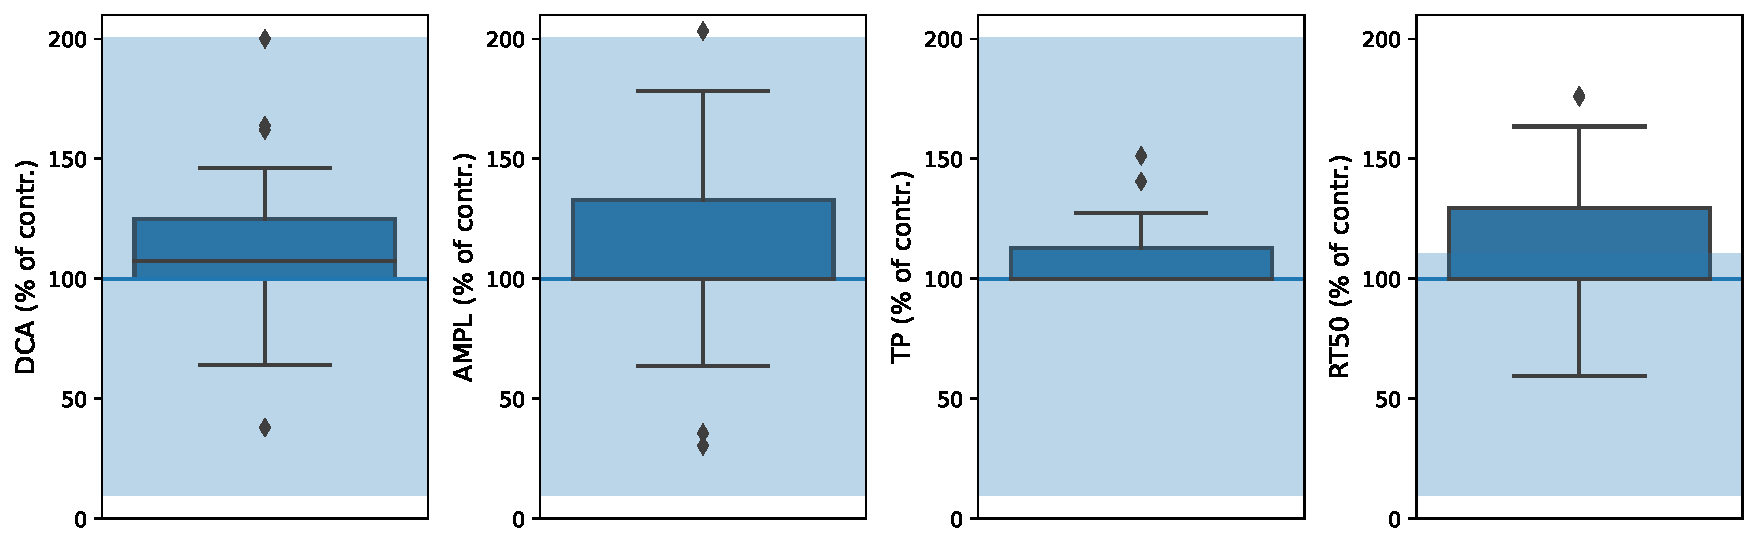
\includegraphics[width=\textwidth]{figures/chapter07/ca_literature_review_all_studies.pdf}
    \caption{Calcium transient parameters' experimental percentage variations' distributions in heart failure rat models (blue boxes). The chosen $\textit{in silico}$ variability for the same parameters is also shown as blue shaded areas.}
    \label{fig:calitdistr}
\end{figure}

\vspace{0.2cm}
For the rest of the mechanics-regulating parameters ($\Caif$, $\betaone$, $\koff$, $\ntrpn$, $\kxb$, $\nxb$, $\trpnf$, $\tref$, $\p$, $\pao$, $\Z$, $\Cone$) the adopted range was $[\SI{50}{\percent},\,\SI{150}{\percent}]$ of the respective control values. This ensured that parameter values were consistent with the variability observed in both literature modelling and experimental studies on both healthy and diastolic heart failure rat models (Tables~\ref{tab:shamranges}--\ref{tab:abranges}), while being symmetric around the baseline value ($\SI{100}{\percent}$). Additional information from local sensitivity analysis studies was used to adjust the $\betaone$ parameter range to be almost twice as big ($[\SI{10}{\percent},\,\SI{200}{\percent}]$ of reference value), as LV features had a limited sensitivity to $\betaone$ in the narrower range. The adopted ranges for the full set of simulator/emulator $16$ input parameters are reported in Table~\ref{tab:finalparranges}.

\begin{table}[ht!]
    \myfloatalign
    \begin{tabularx}{\textwidth}{XXX}
    \toprule
    \tableheadline{Parameter} & \tableheadline{Units}                   & \tableheadline{Range} \\
    \midrule
    $\dca$                    & $\SI{}{\micro\Molar}$                   & $[0.0463,\,0.9264]$ \\
    $\ampl$                   & $\SI{}{\micro\Molar}$                   & $[0.1034,\,2.0681]$ \\
    $\tp$                     & $\SI{}{\milli\second}$                  & $[2.5947,\,51.8947]$ \\
    $\rtf$                    & $\SI{}{\milli\second}$                  & $[4.0081,\,44.0888]$ \\
    $\Caif$                   & $\SI{}{\micro\Molar}$                   & $[1.0861,\,3.2584]$ \\
    $\betaone$                & $-$                                     & $[-3.00,\,-0.15]$ \\
    $\koff$                   & $\SI{}{\per\milli\second}$              & $[0.0257,\,0.0772]$ \\
    $\ntrpn$                  & $-$                                     & $[1.0,\,3.0]$ \\
    $\kxb$                    & $\SI{}{\per\milli\second}$              & $[0.0086,\,0.0258]$ \\
    $\nxb$                    & $-$                                     & $[2.5,\,7.5]$ \\
    $\trpnf$                  & $-$                                     & $[0.1750,\,0.5250]$ \\
    $\tref$                   & $\SI{}{\kilo\pascal}$                   & $[78.03,\,234.10]$ \\
    $\p$                      & $\SI{}{\kilo\pascal}$                   & $[0.1561,\,0.4683]$ \\
    $\pao$                    & $\SI{}{\kilo\pascal}$                   & $[3.5568,\,10.6704]$ \\
    $\Z$                      & $\SI{}{\mmHg\second\per\milli\liter}$   & $[2.8117,\,8.4351]$ \\
    $\Cone$                   & $\SI{}{kPa}$                            & $[0.4571,\,1.3712]$ \\
    \bottomrule
    \end{tabularx}
    \caption{Parameters' ranges used for describing the healthy rat model $16$D input parameter space.}
    \label{tab:finalparranges}
\end{table}


%
%
%
\subsection{Training dataset, emulators, global sensitivity analysis}\label{sec:ch7training_dataset_emulators_global_sensitivity_analysis}
We sampled $14,848$ points from a LHD over the input parameter space $X$ defined in Section~\ref{sec:ch7inputparameterspace}. The simulator was run at these points, and the successfully completed simulations were collected to form the training dataset ($1,299$ points). As the percentage of viable points out of the totally simulated points was low ($\sim\SI{8.7}{\percent}$), we visually and quantitatively inspected the training dataset input parameter space to search for regions which could have been not well represented after training the emulators.

\begin{figure}[ht!]
    \myfloatalign
    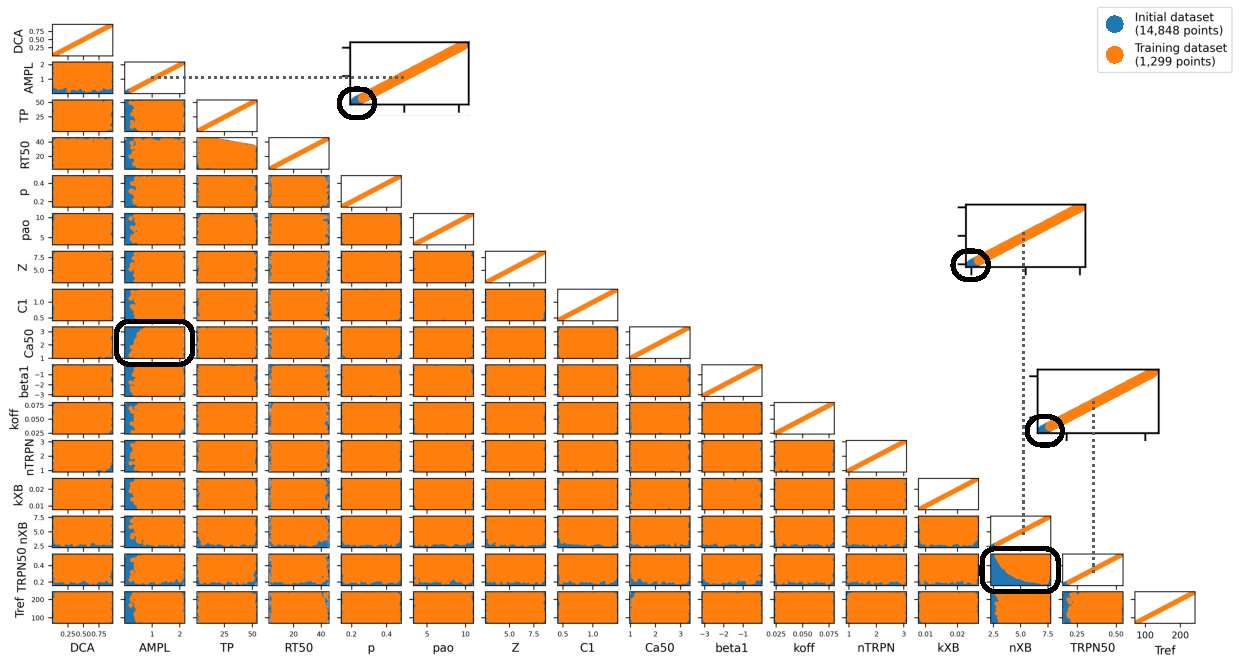
\includegraphics[width=\textwidth]{figures/chapter07/space_examined.pdf}
    \caption{Training dataset visual exploration. The GPEs' training dataset $16$D input parameter space is plotted as a $2$D projection for each pair of parameters (orange dots). The initial space (blue dots) simulated for building the training dataset is plotted in the same manner to highlight regions which are not covered by the training dataset.}
    \label{fig:trainingspaceexamined}
\end{figure}

\vspace{0.2cm}\noindent
Figure~\ref{fig:trainingspaceexamined} shows that indeed there are regions of the input parameter space which are not covered by the training dataset due to simulator failures at points from these regions. In particular, $\ampl$, $\nxb$ and $\trpnf$ parameters could not take values below $0.2$, $2.8$ and $0.195$, respectively (simulated values were $>0.1$, $>2.5$ and $>0.175$, respectively). This is consistently observed no matter the value of the other parameter points' components, concluding that there are $1$-dimensional portions of the space which were not covered by the training dataset. $2$-dimensional portions of the space which were not covered are also present. These involve $\ampl$-vs-$\Caif$ and $\nxb$-vs-$\trpnf$ parameters' interactions. Specifically, low $\ampl$ values could not co-exist with high $\Caif$ values, this is because high thin filament $\Ca$ sensitivities rapidly activate the myofilament but the small amount of available intracellular $\Ca$ during systole is not enough to sustain contraction. Also, low $\nxb$ values could not co-exist with low $\trpnf$ values, this is because they decrease the cross-bridges steady-state degree of cooperativity and sensitivity to bound $\Ca$-TnC complexes, making it hard for cross-bridges to form and to generate enough tension for the heart to contract.

\vspace{0.2cm}\noindent
In order to provide an estimate of the percentage area out of the total initial space area which was covered by the training dataset, we calculated for each parameter the percentage of final covered portion of its initial full $1$D interval. We then multiplied all the percentage values obtained across the full set of input parameters, resulting in parameters covering $>\SI{80}{\percent}$ of the full parameter space.

\vspace{0.2cm}
Univariate GPEs, defined as in Section~\ref{sec:ch3gaussianprocessemulation}, were used to predict each of the $16$ LV output features, and the GPE model hyperparameters were jointly optimised during training by maximisation of the model log marginal likelihood (equation~\eqref{eq:logmarginallikelihood}). The accuracy and adequacy of being used as a surrogate model for each of the resulting $16$ trained GPEs were evaluated using the $R^2$-score regression metric and the $ISE_2$, as described in Section~\ref{sec:ch3regressionaccuracy}. GPEs' implementation and training were performed using GPErks~\cite{GPErks:2021}.

\vspace{0.2cm}
To study the input parameters' impact on the output LV features' total variance we performed a GSA using the trained GPEs. Model outputs' sensitivity to model inputs was characterised by Sobol' first-order and total effects. These were estimated using \texttt{SALib}~\cite{Herman:2017}. GPErks~\cite{GPErks:2021} was used to incorporate GPEs' full posterior distribution samples to account for emulators' uncertainty in Sobol' indices estimates, by following the second emulation-based approach of equations~\eqref{eq:emulpostsamplesgsa1}--\eqref{eq:emulpostsamplesgsa2}, presented in Section~\ref{sec:ch3emulatorbasedestimates}. Parameters whose Sobol' indices' distributions' expectation was below the threshold $0.01$ were determined to have negligible effects.


%
%
%
\subsection{Building a model of the $20$-week old obese ZSF1 rat}\label{sec:ch7building_a_model_of_the_20_week_old_obese_zsf1_rat}
To create a model of the ZSF1 rat, we re-fitted SHAM model parameters using HM technique (Section~\ref{sec:ch3historymatching}), using the maximum implausibility measure (equation~\eqref{eq:maximplmeasure}) across multiple target features, with the model discrepancy term (and its corresponding variance) set to zero in equation~\eqref{eq:implmeasure}. We first applied the experimental percentage variability observed in the ZSF1 rat studies when going from control to diseased rats (Table~\ref{tab:obesezsf1data}) to the SHAM rat model corresponding features' baseline values (Table~\ref{tab:shamabbestfitfeatvalues}). We then tried to match the resulting experimental variability during HM. As $\textrm{EF}$ did not change significantly in any experiment, we matched for this feature an experimental variability of $\SI{100}{\percent}\pm\SI{0}{\percent}$ (i.e. no change).

\vspace{0.2cm}
To understand which of the $16$ model parameters (Table~\ref{tab:paramswithdeffinal}) could undergo re-fitting, we collected evidence for changing each of them from literature studies. In ZSF1 rats, the intracellular $\Ca$ transient was shown to have increased diastolic concentrations and decreased/unaltered amplitudes at multiple frequencies ($1$-$\SI{4}{\Hz}$-paced cells)~\cite{Miranda-Silva:2020, Abdellatif:2021}, so we fitted $\dca$ and $\ampl$ parameters. As the observed changes in time to peak $\Ca$ and time to $\Ca$ half-relaxation could not be extrapolated at physiological pacing rates, $\tp$ and $\rtf$ parameters were kept fixed. Also, end-diastolic pressure~\cite{Abdellatif:2016, Bowen:2017, Hamdani:2013, Hohendanner:2018, Lai:2016, Leite:2015, Leite:2015*a, Leite:2019, Salah:2018, Schmederer:2018} and cardiac tissue stiffness~\cite{Hamdani:2013, Abdellatif:2016, Van-Dijk:2016, Salah:2018, Schmederer:2018, Leite:2019, Davila:2019, Nguyen:2020} were consistently shown to be increased w.r.t control, so we fitted $p$ and $C_1$ parameters. Furthermore, there was evidence for an increase in arterial systolic pressure~\cite{Cuijpers:2020} and aortic characteristic impedance~\cite{Leite:2019}, therefore parameters $\pao$, $Z$ were selected for optimisation as well. As there were no statistically significant changes in the reported values of myocardial active contraction in ZSF1 rats~\cite{Deel:2017, McCain:2014, Hersch:2013}, we assumed that sarcomere properties remained unchanged (i.e. $\Caif$, $\beta_1$, $\koff$, $\ntrpn$, $\kxb$, $\nxb$, $\trpnf$, $\tref$ parameters were not fitted). Although the ZSF1 rats all developed LV hypertrophy as shown by increased cardiac fibrosis, collagen type III fibres and cardiomyocyte size (increased LV mass and indexes of LV mass such as LV $+$ IVS weights / tibial length), this was not always (e.g.~\cite{Van-Dijk:2016, Schmederer:2018}) accompanied by an increase in LV wall thickness in male ZSF1 rats. Moreover, half of the ZSF1 rat studies~\cite{Hamdani:2013, Leite:2015, Leite:2015*a, Leite:2019, Abdellatif:2016, Lai:2016, Van-Dijk:2016, Nguyen:2020} showed no LV dilation as appraised by indexed end-diastolic volumes (preserved EDVi), which we translated into a no change in the biventricle size/shape. To summarise, $6$ out of $16$ SHAM rat model parameters were re-fitted to build the ZSF1 rat model while keeping the other parameters fixed to reference values.

\vspace{0.2cm}
We therefore sampled $400,000$ $NROY$ points from a LHD in the input parameter space $X$ (Section~\ref{sec:ch7inputparameterspace}), which was \textit{a priori} constrained according to the above-mentioned literature evidence. This means that for parameters that were observed to significantly vary in one specific direction, the corresponding $1$D slice of the full hypercube was cut in two equal parts and only the half which corresponded to the correct direction of change from the reference parameter value was used to generate the initial hypercube. Parameters not selected for optimisation (no significant change when going from control to diseased ZSF1 rats), had their $1$D slices fixed to a single value instead (the SHAM rat reference value), effectively reducing the initial hypercube of $1$ dimension for each of them. The resulting sampled $NROY$ space was therefore a $6$-dimensional space. The $NROY$ points were then tested against an implausibility criterion with $I_{\,\textrm{cutoff}}=3.0$.


%
%
%
\subsection{In silico recovering the ZSF1 rat towards healthy conditions}\label{sec:ch7in_silico_recovering_the_zsf1_rat_towards_healthy_conditions}
The ZSF1 rat model we are building will constitute a virtual platform to better understand pathophysiological mechanisms of a diseased, HFpEF animal model. We aim at using this platform to identify cellular properties that can be manipulated to recover the ZSF1 rat towards an healthy condition. By ``recover" we mean to bring the altered LV features' values of the ZSF1 rat model back to the values of the SHAM rat model. We will do so by specifically targeting different subsets of model parameters to \textit{in silico} represent different possible pharmacological compounds' mechanisms of action.

\vspace{0.2cm}
For this purpose, starting from the built ZSF1 rat model, we re-fitted model parameters to go back to the initial, healthy state of the SHAM rat model, matching the \textit{in silico} variability observed for the LV function in the SHAM rat model (Section~\ref{sec:ch4modelfitting}, Figure~\ref{fig:simulatormatchtoexpvar}), summarised in Table~\ref{tab:targetfeatsforrecovery}. A preliminary sketch of the recovery process is provided in Figure~\ref{fig:zsf1andshamrefwithvar}.

\begin{table}[ht!]
    \myfloatalign
    \begin{tabularx}{\textwidth}{XXX}
    \toprule
    \tableheadline{LV feature} & \tableheadline{Units}                  & \tableheadline{Synthetic variability} \\
    \midrule
    $\textrm{EDV}$             & $\SI{}{\micro\liter}$                  & $498.22 \pm 13.21$ \\
    $\textrm{ESV}$             & $\SI{}{\micro\liter}$                  & $185.12 \pm  4.08$ \\
    $\textrm{PeakP}$           & $\SI{}{\kilo\pascal}$                  & $ 16.14 \pm  0.49$ \\
    $\textrm{maxdP}$           & $\SI{}{\kilo\pascal\per\milli\second}$ & $  0.95 \pm  0.04$ \\
    $\textrm{Tau}$             & $\SI{}{\milli\second}$                 & $  6.52 \pm  0.40$ \\
    \bottomrule
    \end{tabularx}
    \caption{SHAM rat model \textit{in silico} variability for the LV features used as targets for ZSF1 rat model recovery. Target mean and standard deviation LV features' values to be matched for recovering the ZSF1 rat.}
    \label{tab:targetfeatsforrecovery}
\end{table}

\begin{figure}[ht!]
    \myfloatalign
    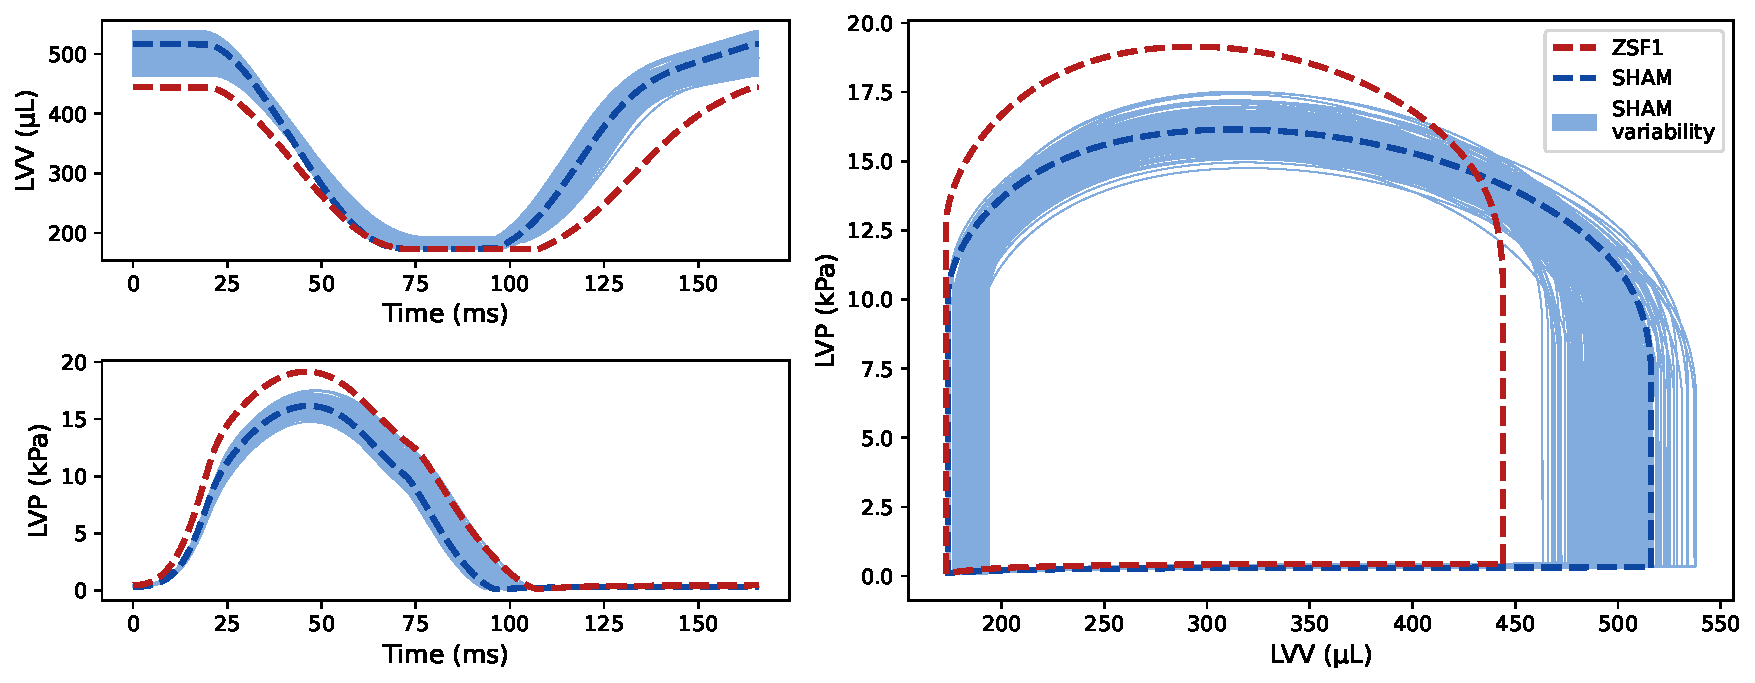
\includegraphics[width=\textwidth]{figures/chapter07/zsf1_vs_sham_last_wave_plus_ref.pdf}
    \caption{ZSF1 rat model recovery towards SHAM rat model. ZSF1 rat (red) and SHAM rat (blue) models' LV pressure and volume transients and PV loops are plotted with dashed lines. SHAM model \textit{in silico} variability is also represented by a cloud of thin blue full lines. Black arrow represents the direction of recovery.}
    \label{fig:zsf1andshamrefwithvar}
\end{figure}

\vspace{0.2cm}
The LV features we aimed to recover were $\textrm{EDV}$, $\textrm{ESV}$, $\textrm{PeakP}$, $\textrm{maxdP}$, $\textrm{Tau}$. The groups of parameters selected for optimisation were: $\Ca$ transient ($\dca$, $\ampl$, $\tp$, $\rtf$), thin filament ($\Caif$, $\betaone$, $\koff$, $\ntrpn$), thick filament ($\kxb$, $\nxb$, $\trpnf$, $\tref$) and the three groups combined, labelled, respectively, as "Ca'', "TNF'', "TKF'' and "CaMYO''. We performed a separate HM for each group. This required to build a specific set of emulators to be used each time.

\vspace{0.2cm}
For each group of $D$ parameters $\mathbf{p}=(p_1,\,\dots,\,p_D)$, we trained one univariate GPE for each of the target LV features to replace the deterministic map
%
\begin{align}
    f\colon\mathbb{R}^D &\to \mathbb{R} \\
    \mathbf{p} &\mapsto f_{simul}(\mathbf{p},\,(p_{D+1}^{\textrm{ZSF1}},\dots,\,p_{16}^{\textrm{ZSF1}}))=y
\end{align}

\vspace{0.2cm}\noindent
with a probabilistic surrogate to predict the LV feature value $y\in\mathbb{R}$ for a given parameter set $\mathbf{p}\in\mathbb{R}^D$. The training datasets were built by sampling points ($512$ for Ca, TNF, TKF groups and $2048$ for CaMYO group) from a LHD over the restricted, $D$-dimensional parameter space and by running the full simulator $f_{simul}$ (equation~\eqref{eq:fsimulfinal}) at these points while keeping all the remaining parameters $(p_{D+1}^{\textrm{ZSF1}},\dots,\,p_{16}^{\textrm{ZSF1}})$ fixed to the ZSF1 reference values. 


%
%
%
\section{Results}\label{sec:ch7results}


%
%
%
\subsection{Model emulators and output sensitivities}\label{sec:ch7model_emulators_and_output_sensitivities}
The GPEs' cross-validation mean accuracy is reported in Table~\ref{tab:gpescoresfinal}. The mean $R^2$ score was $>0.9$ for $4$ out of $14$ emulated features, while for all the other features ($10$ out of $14$) it was ranging between $0.45$ and $0.9$. The lowest values were obtained for features representing timings ($0.51$, $0.50$, $0.49$ for IVCT, Tdiast, Tpeak, respectively) but not for features representing magnitudes (lowest was $0.76$ for EF). On the other hand, the $ISE_{2}$ was $>0.9$ for all the features. This suggested that the GPEs' posterior distributions' variance was correctly increasing to account for a greater uncertainty in the point-wise predictions coming from less accurate emulators.

\begin{table}[ht!]
    \myfloatalign
    \begin{tabularx}{\textwidth}{XXX}
    \toprule
    \tableheadline{LV feature} & \tableheadline{$R^2$} & \tableheadline{$ISE_2 (\SI{}{\percent})$} \\
    \midrule
    $\textrm{EDV}$             & $0.9437\pm 0.0089$    & $98.38\pm 0.61$ \\
    $\textrm{ESV}$             & $0.8344\pm 0.0227$    & $98.92\pm 0.75$ \\
    $\textrm{SV}$              & $0.7937\pm 0.0228$    & $98.92\pm 0.66$ \\
    $\textrm{EF}$              & $0.7627\pm 0.0051$    & $98.77\pm 0.45$ \\
    $\textrm{IVCT}$            & $0.5190\pm 0.0579$    & $93.46\pm 1.19$ \\
    $\textrm{ET}$              & $0.7900\pm 0.0248$    & $97.15\pm 1.49$ \\
    $\textrm{IVRT}$            & $0.7467\pm 0.0480$    & $97.54\pm 1.02$ \\
    $\textrm{Tdiast}$          & $0.5047\pm 0.0226$    & $94.53\pm 1.07$ \\
    $\textrm{PeakP}$           & $0.8942\pm 0.0114$    & $98.61\pm 0.79$ \\
    $\textrm{Tpeak}$           & $0.4921\pm 0.0362$    & $94.30\pm 1.15$ \\
    $\textrm{ESP}$             & $0.9556\pm 0.0074$    & $98.07\pm 0.69$ \\
    $\textrm{maxdP}$           & $0.9448\pm 0.0087$    & $98.46\pm 0.81$ \\
    $\textrm{mindP}$           & $0.9008\pm 0.0121$    & $97.84\pm 1.10$ \\
    $\textrm{Tau}$             & $0.8213\pm 0.0168$    & $96.69\pm 0.72$ \\
    \bottomrule
    \end{tabularx}
    \caption{GPEs' accuracy. The GPEs' accuracy was evaluated using the average $R^{2}$ score and $ISE_2$ obtained with a $5$-fold cross-validation. Values are reported as mean$\pm$std.}
    \label{tab:gpescoresfinal}
\end{table}

\begin{figure}[ht!]
    \myfloatalign
    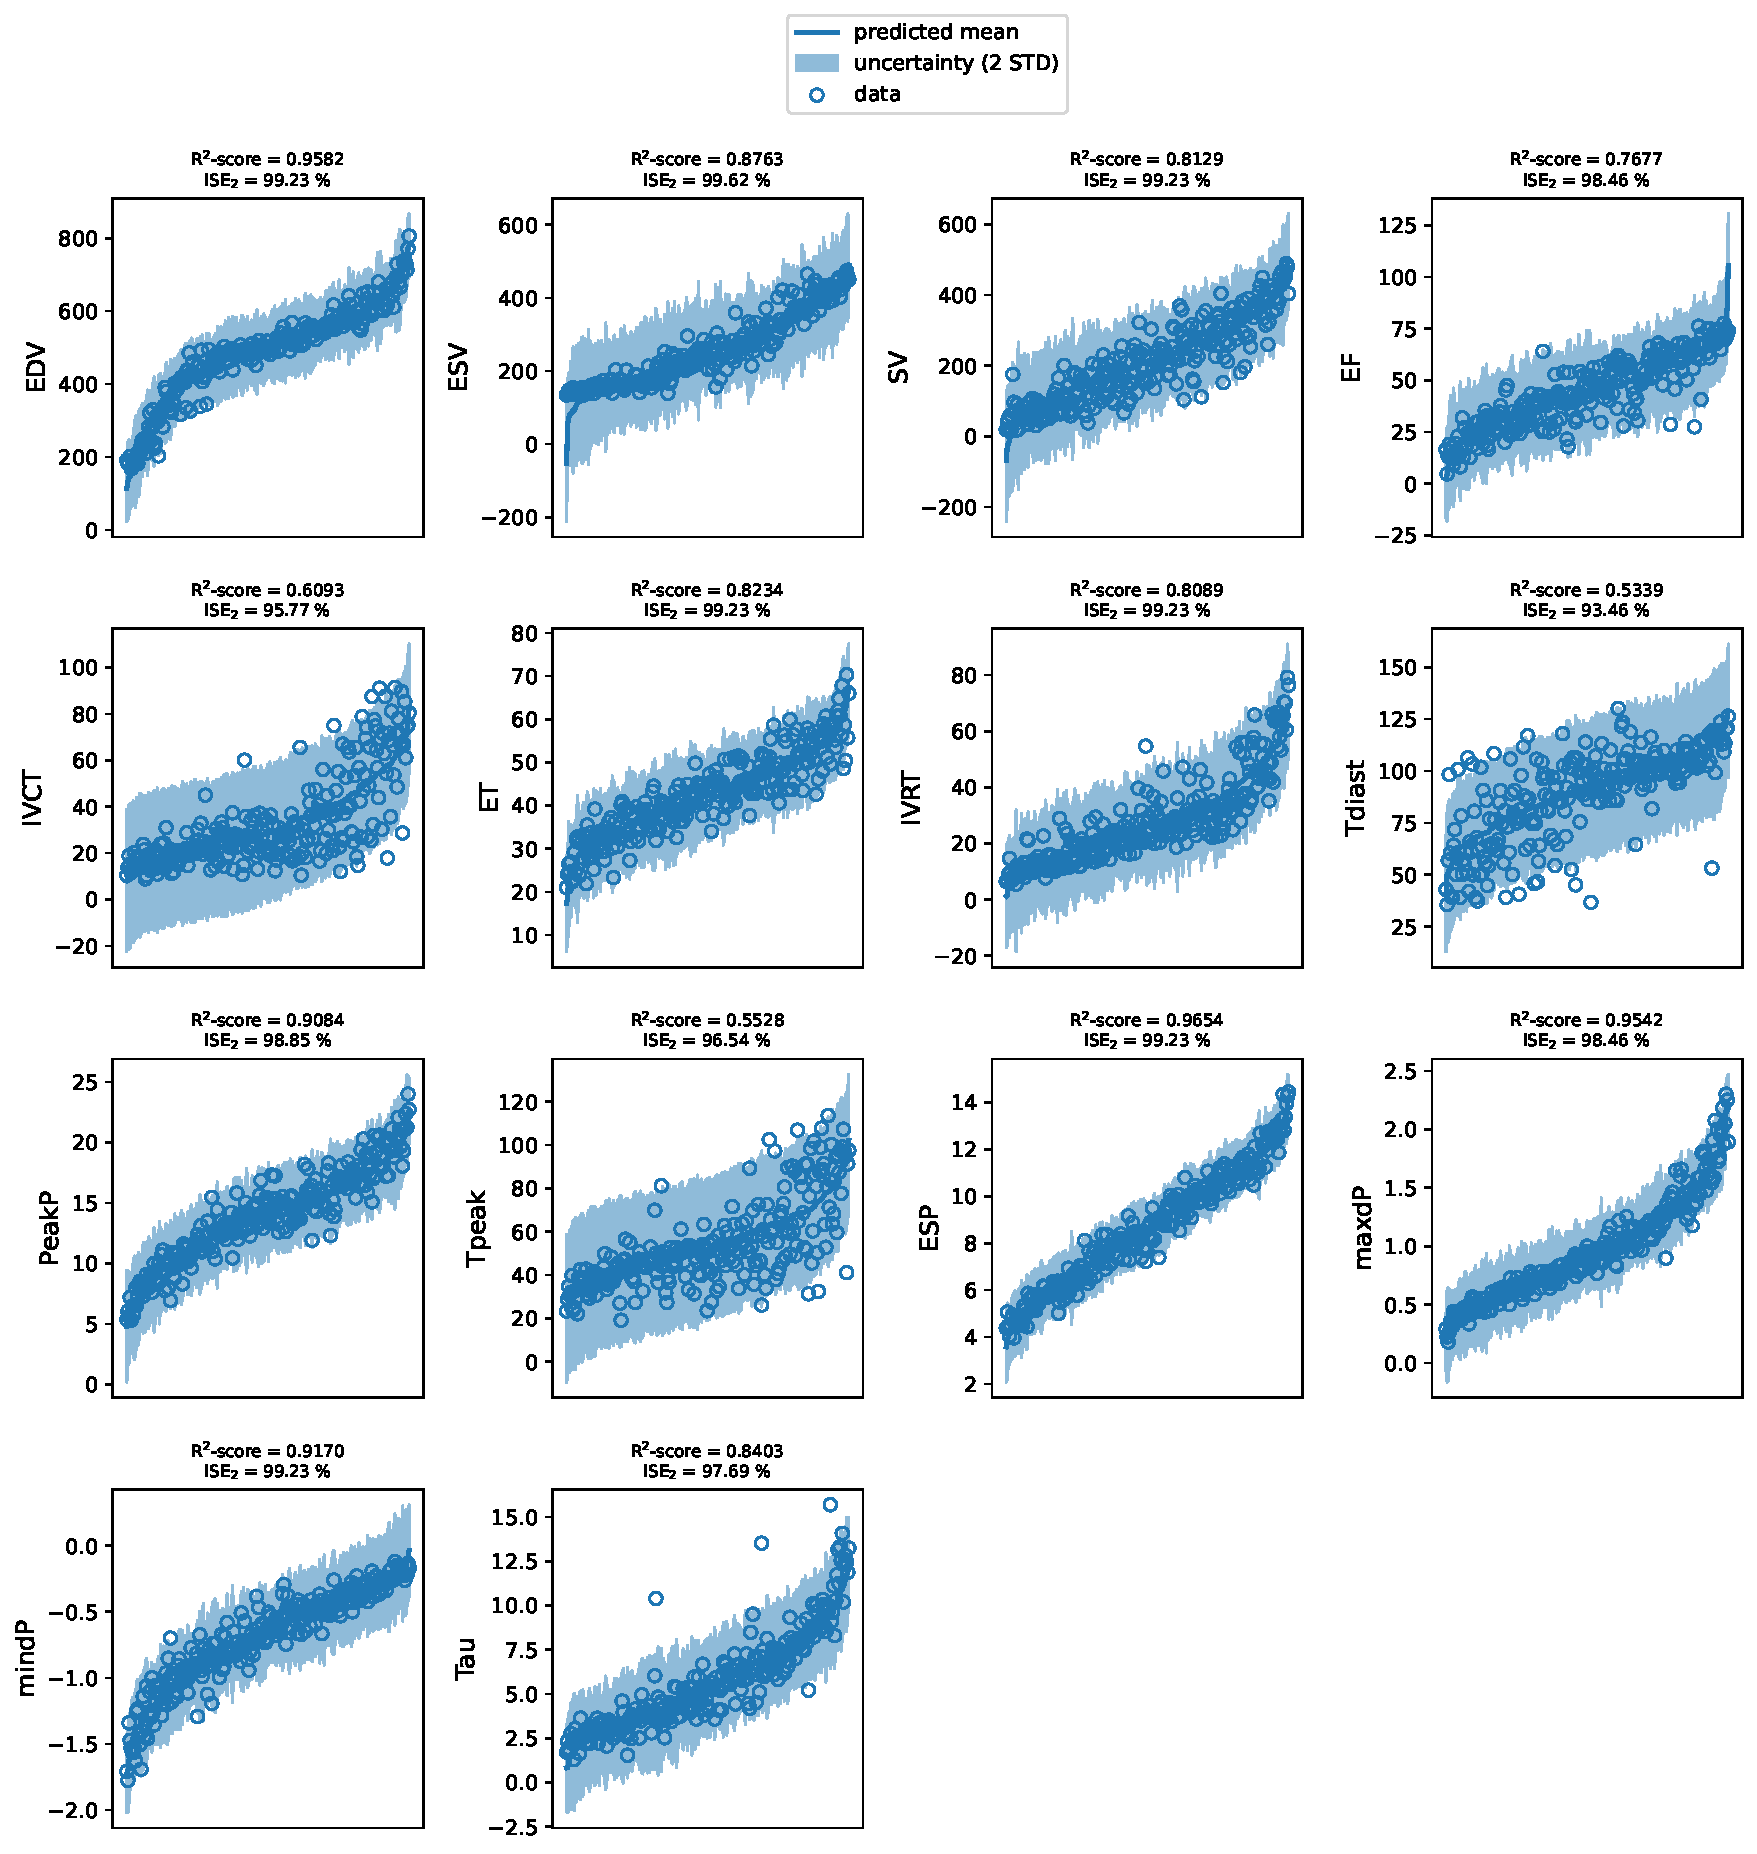
\includegraphics[width=\textwidth]{figures/chapter07/bgpes_vs_bsplit_16p.pdf}
    \caption{For each LV feature, the GPE with the highest $R^2$ split test score is used to make predictions at the respective left-out subset of test points. Predictions are sorted in ascending order for the sake of a better visualisation and joined with a thick blue line, and the respective observations (empty dots) are sorted accordingly. $2$ STD confidence intervals (shaded regions) are also plotted around predicted mean lines.}
    \label{fig:bgpevsbsplitfinal}
\end{figure}

\vspace{0.2cm}
In Figure~\ref{fig:s1stdonutfinal}, the calculated Sobol' first-order effects are reported for all the $14$ LV features. In Section~\ref{sec:ch7in_silico_recovering_the_zsf1_rat_towards_healthy_conditions}, we have identified groups of parameters which regulate a specific cellular component ($\Ca$ transient, thin filament, thick filament) and which we will re-fit to mimic possible pharmacological interventions at the cell level to \textit{in silico} treat rat HFpEF. To determine which of these parameter sets has the greatest impact overall on whole heart cardiac mechanics, we ranked the parameters according to their total effects from the one that affected the highest number (and by the highest amount) to the one that affected the lowest number (and by the lowest amount) of LV features. The obtained ranking is presented in Table~\ref{tab:paramsranking}. We thus divided the $16$ parameters in $4$ sub-categories according to which specific part of the multi-scale model they regulated, the first three being the above-mentioned parameter groups while the last group describing passive material and boundary conditions properties (labelled as "BC''), with $4$ parameters in each category. By summation of the parameters' individual ranks within each category we were able to classify the groups according to how important they are in explaining the variance across output variables: the lower the sum, the higher the importance. We found that the $\Ca$ transient is the most important input of the multi-scale model, immediately followed by the thin filament and the thick filament. The boundary conditions were found not to play an important role in this model (ranked fourth). To summarise, altering preload and afterload were predicted to have a secondary impact on the overall cardiac function, with cellular properties being the dominant regulators of cardiac function.

% \begin{figure}[ht!]
%     \myfloatalign
%     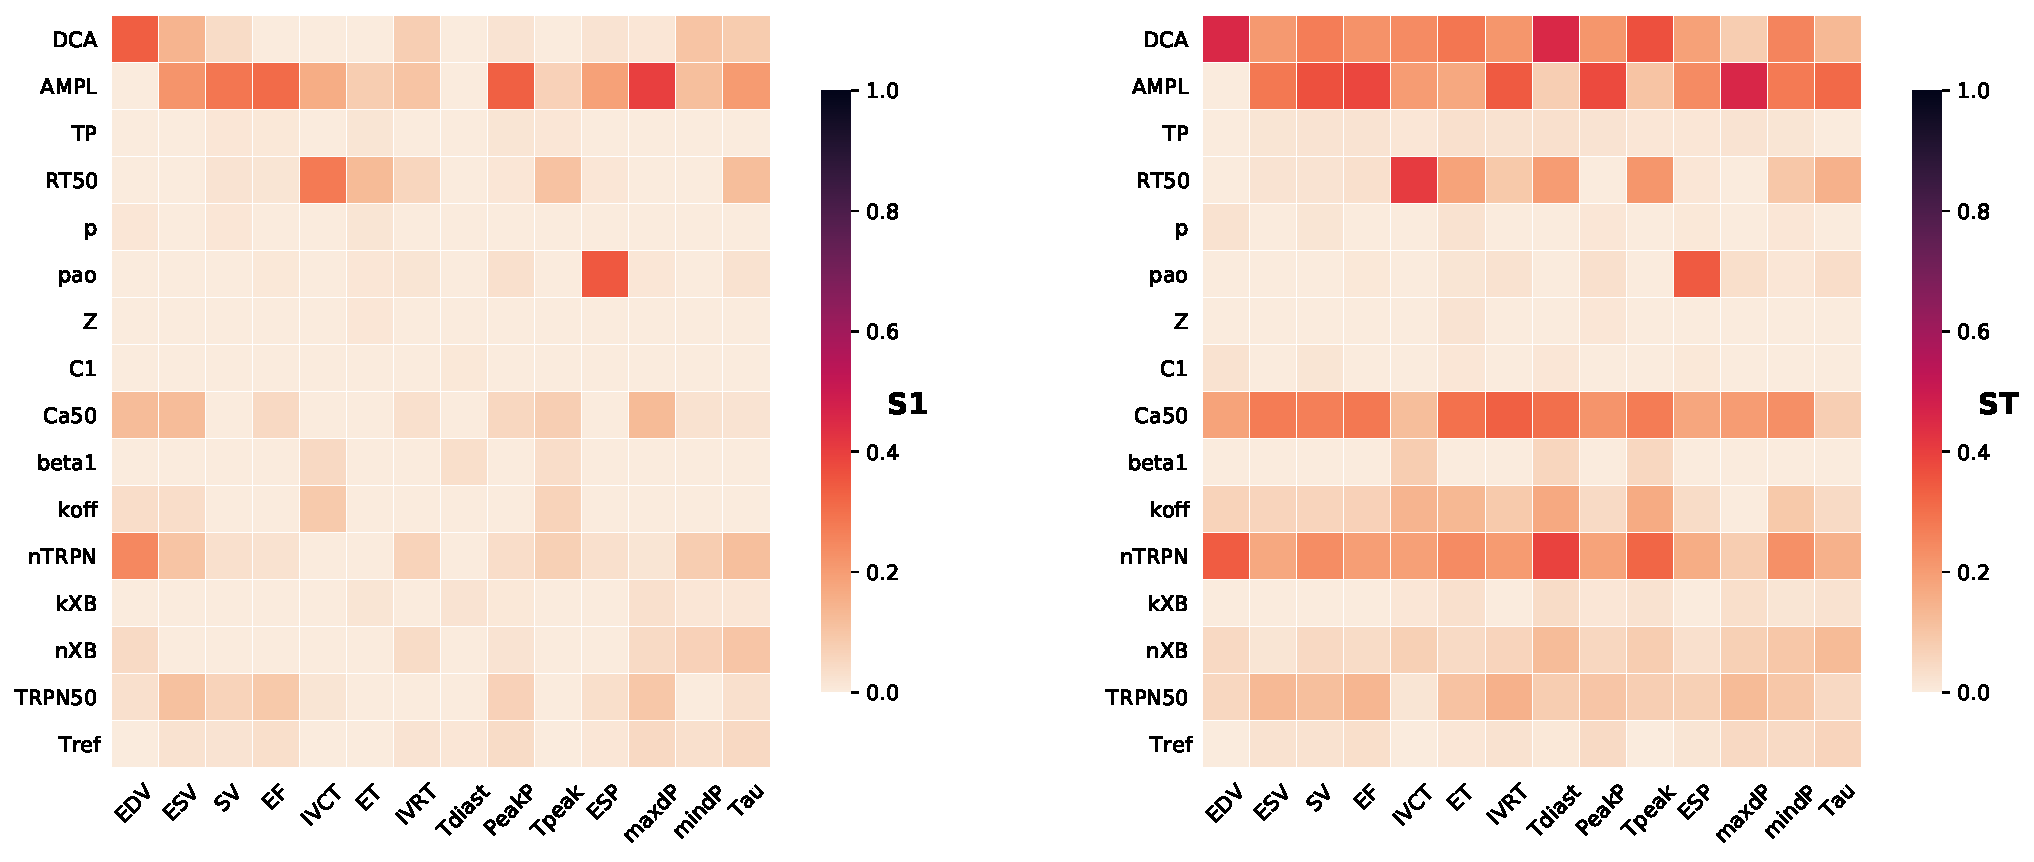
\includegraphics[width=\textwidth]{figures/chapter07/gsa_16p_heatmap_S1_ST.pdf}
%     \caption{Sobol' first-order (S1) and total effects (ST). The contribution of each parameter (Table~\ref{tab:paramswithdeffinal}) by itself (S1) or jointly with the other parameters (ST) into explaining the total variance of each LV feature (Tables~\ref{tab:lvfeatures}--\ref{tab:lvfeaturesfinal}) is expressed as Sobol' indices ranging from $0$ (no effect) to $1$ (maximal effect).}
%     \label{fig:s1stheat}
% \end{figure}

\begin{figure}[ht!]
    \myfloatalign
    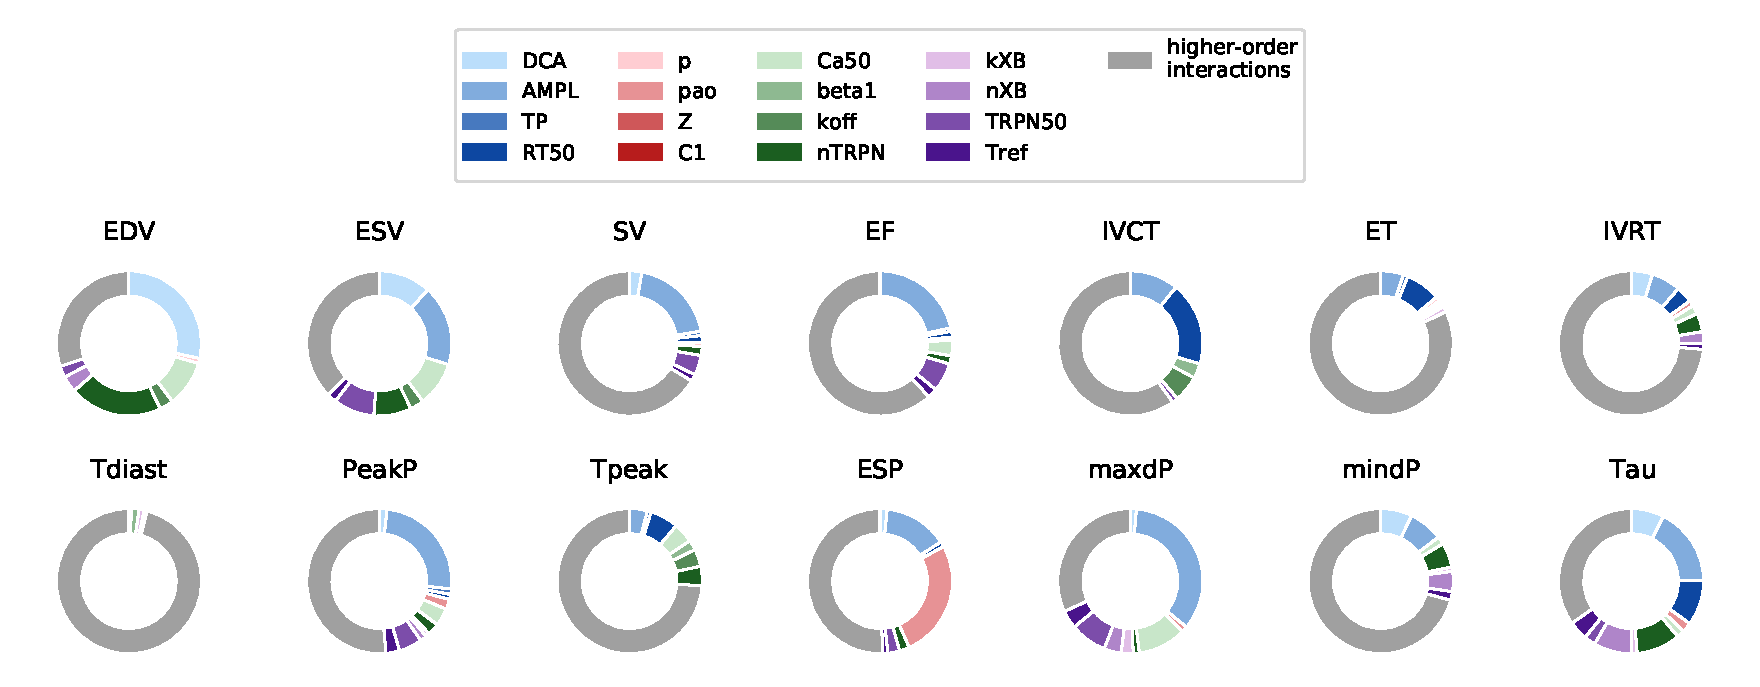
\includegraphics[width=\textwidth]{figures/chapter07/gsa_16p_donut_S1.pdf}
    \caption{The impact of calcium dynamics, sarcomere, tissue and boundary conditions properties on organ-scale LV features in the healthy rat. The contribution of each parameter is represented by its Sobol' main effect. For each LV feature, higher-order interactions (coloured in grey) are represented by the sum of all total effects minus the sum of all main effects.}
    \label{fig:s1stdonutfinal}
\end{figure}

\begin{table}[ht!]
    \myfloatalign
    \begin{tabularx}{\textwidth}{lXXX}
    \toprule
    \tableheadline{Group} & \tableheadline{Parameter} & \tableheadline{Rank} & \tableheadline{Score}\\
    \midrule
    \multirow{4}{*}{\parbox{4.0cm}{Calcium transient \\ (Ca)}} & $\dca$     & $1$ & \multirow{4}{*}{22} \\
    & $\ampl$    & $3$ \\
    & $\tp$      & $10$ \\
    & $\rtf$     & $8$ & \\
    \midrule
    \multirow{4}{*}{\parbox{4.0cm}{Thin filament \\ (TNF)}} & $\Caif$    & $2$ & \multirow{4}{*}{26} \\
    & $\betaone$ & $14$ & \\
    & $\koff$    & $6$ & \\
    & $\ntrpn$   & $4$ & \\
    \midrule
    \multirow{4}{*}{\parbox{4.0cm}{Thick filament \\ (TKF)}} & $\kxb$     & $12$ & \multirow{4}{*}{33} \\
    & $\nxb$     & $7$ & \\
    & $\trpnf$   & $5$ & \\
    & $\tref$    & $9$ & \\
    \midrule
    \multirow{4}{*}{\parbox{4.0cm}{Boundary conditions \\ (BC)}} & $\p$       & $13$ & \multirow{4}{*}{55} \\
    & $\pao$     & $11$ & \\
    & $\Z$       & $16$ & \\
    & $\Cone$    & $15$ & \\
    \bottomrule
    \end{tabularx}
    \caption{Parameters ranking according to their influence on the model output total variance. A rank is assigned to each parameter according to how much it impacts the model output total variance. Parameter groups are assigned a score given by the sum of the ranks of their member parameters. This score reflects the importance of the group as an input for the multi-scale model.}
    \label{tab:paramsranking}
\end{table}


%
%
%
\subsection{Personalised healthy rat heart model validation using emulators}\label{sec:ch7personalised_healthy_rat_model_validation_using_emulators}
Having available trained emulators that can map $\Ca$ transient properties to LV function allowed us to further validate the SHAM rat model against experimentally observed CiPA compounds' effects by following the same approach of Section~\ref{sec:ch6validating_the_personalised_healthy_rat_heart_model}. However, in this case we replaced the simulator with the emulator in the last validation step when LV features' dose-response curves are calculated. In particular, the perturbed $\Ca$ transients, obtained when simulating the compounds' effects at cellular level, were first encoded by the $4$ parameters, and then these parameters were mapped to LV features' values using the emulators while fixing the other $12$ parameters of the input vector to the healthy baseline values. Predicted LV pressure features' dose-response curves are shown in Figure~\ref{fig:LVfeatsalldrugsrespcurves}.

\begin{figure}[ht!]
    \myfloatalign
    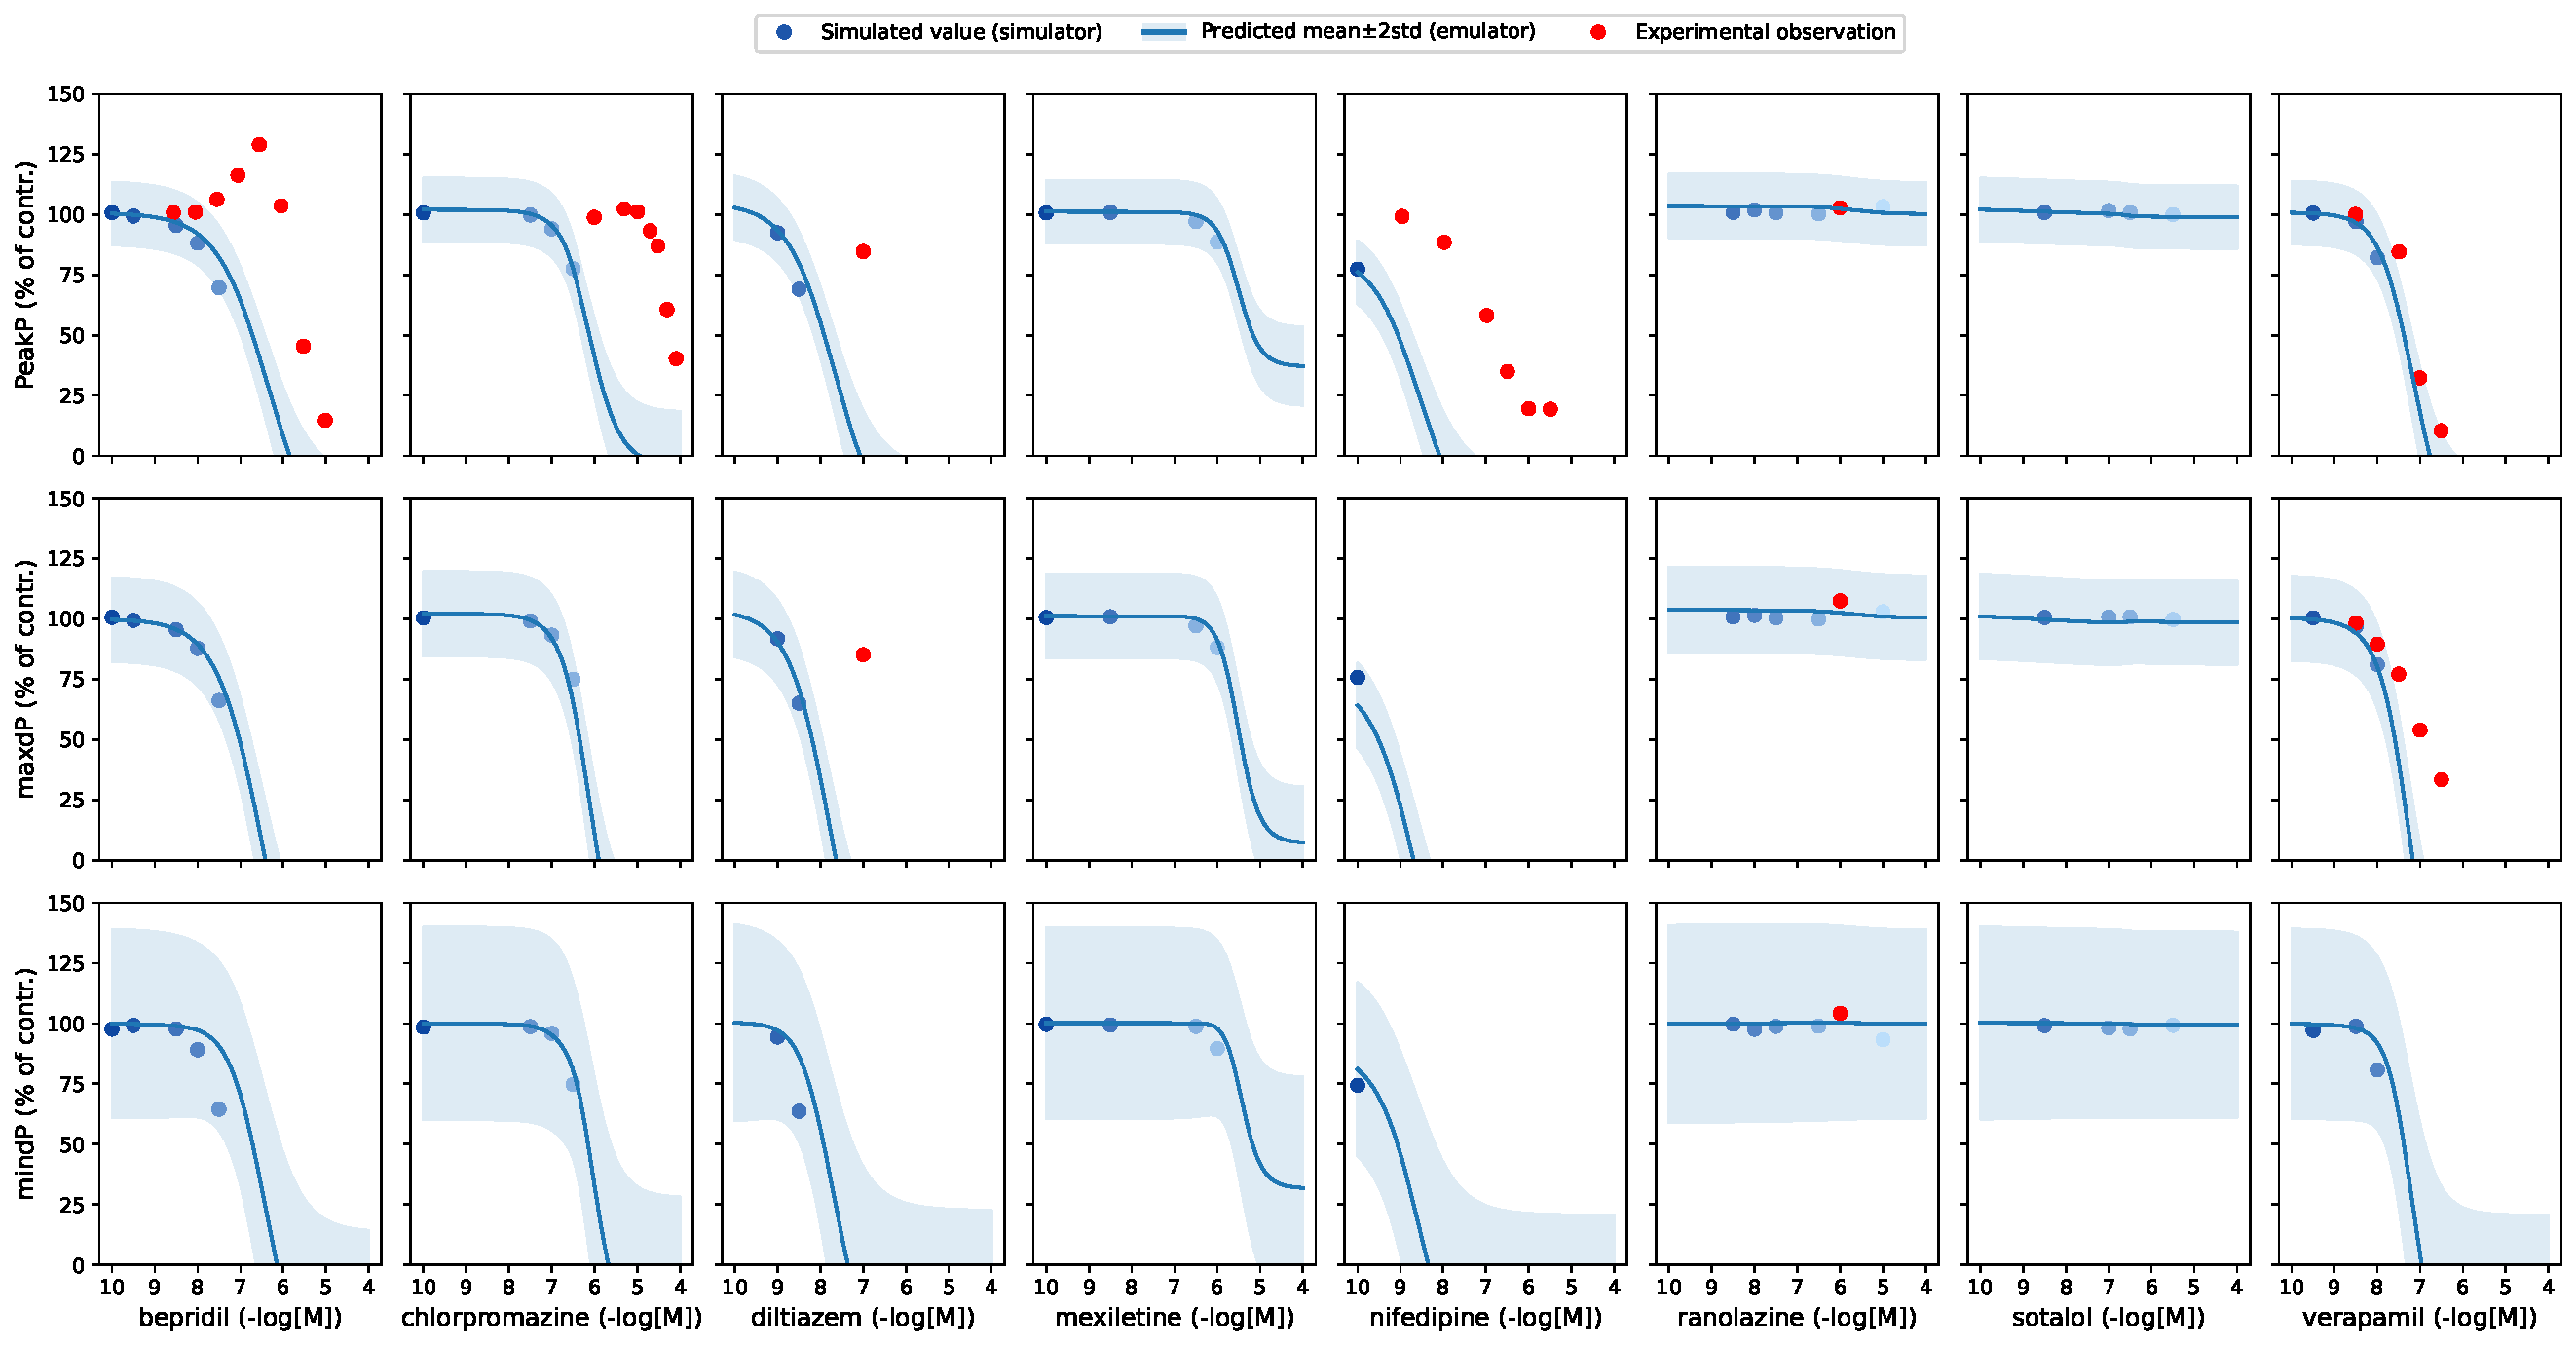
\includegraphics[width=\textwidth]{figures/chapter07/simulated_and_emulated_cipa_compounds_effects_on_lv_pressure_features_with_exp_data.pdf}
    \caption{LV pressure features' dose-response curves for the eight CiPA compounds. Simulated (dots in blue variants, colour-coded with the compound doses), emulated (full lines and shaded areas in blue) and experimentally observed (dots in red) PeakP, maxdP and mindP features' values are given as percentages of the respective control values. Experimental data taken from~\cite{Amsterdam:1988} (bepridil and verapamil -- PeakP), \cite{Langslet:1971} (chlorpromazine, PeakP), \cite{Koltai:1989} (diltiazem -- PeakP and maxdP), \cite{Saponara:2007} (nifedipine -- PeakP), \cite{Wang:2007} (ranolazine -- PeakP, maxdP and mindP), \cite{Kolar:1990} (verapamil -- maxdP).}
    \label{fig:LVfeatsalldrugsrespcurves}
\end{figure}

\vspace{0.2cm}
In Figure~\ref{fig:LVfeatsalldrugsrespcurves}, we can see that the emulators correctly predict the same LV features' percentage variation from reference trends observed when using the simulator (Figure~\ref{fig:LVRVfeatsalldrugsrespcurves}). Therefore, the same conclusions about the simulator matching qualitative/quantitative experimental observations can be extended to the emulators as well.


%
%
%
\subsection{The ZSF1 rat model}\label{sec:ch7the_zsf1_rat_model}
The first wave of the HM procedure for building the ZSF1 rat model is displayed in Figure~\ref{fig:w1zsf1rat}. $47,097$ points (corresponding to $\SI{11.77}{\percent}$ of all the points tested against the implausibility criterion) were deemed non-implausible. The simulator (equation~\eqref{eq:fsimulfinal}) was then run at a subset of $1024$ $X_{NIMP}$ points to see if the respective simulation output was correctly matching the experimentally observed value for each LV feature under study. This is illustrated in Figure~\ref{fig:w1bestzsf1model}. Since all the simulated features' values already fell between $3$ standard deviations from the respective experimental mean values, we concluded the HM.

\begin{figure}[ht!]
    \myfloatalign
    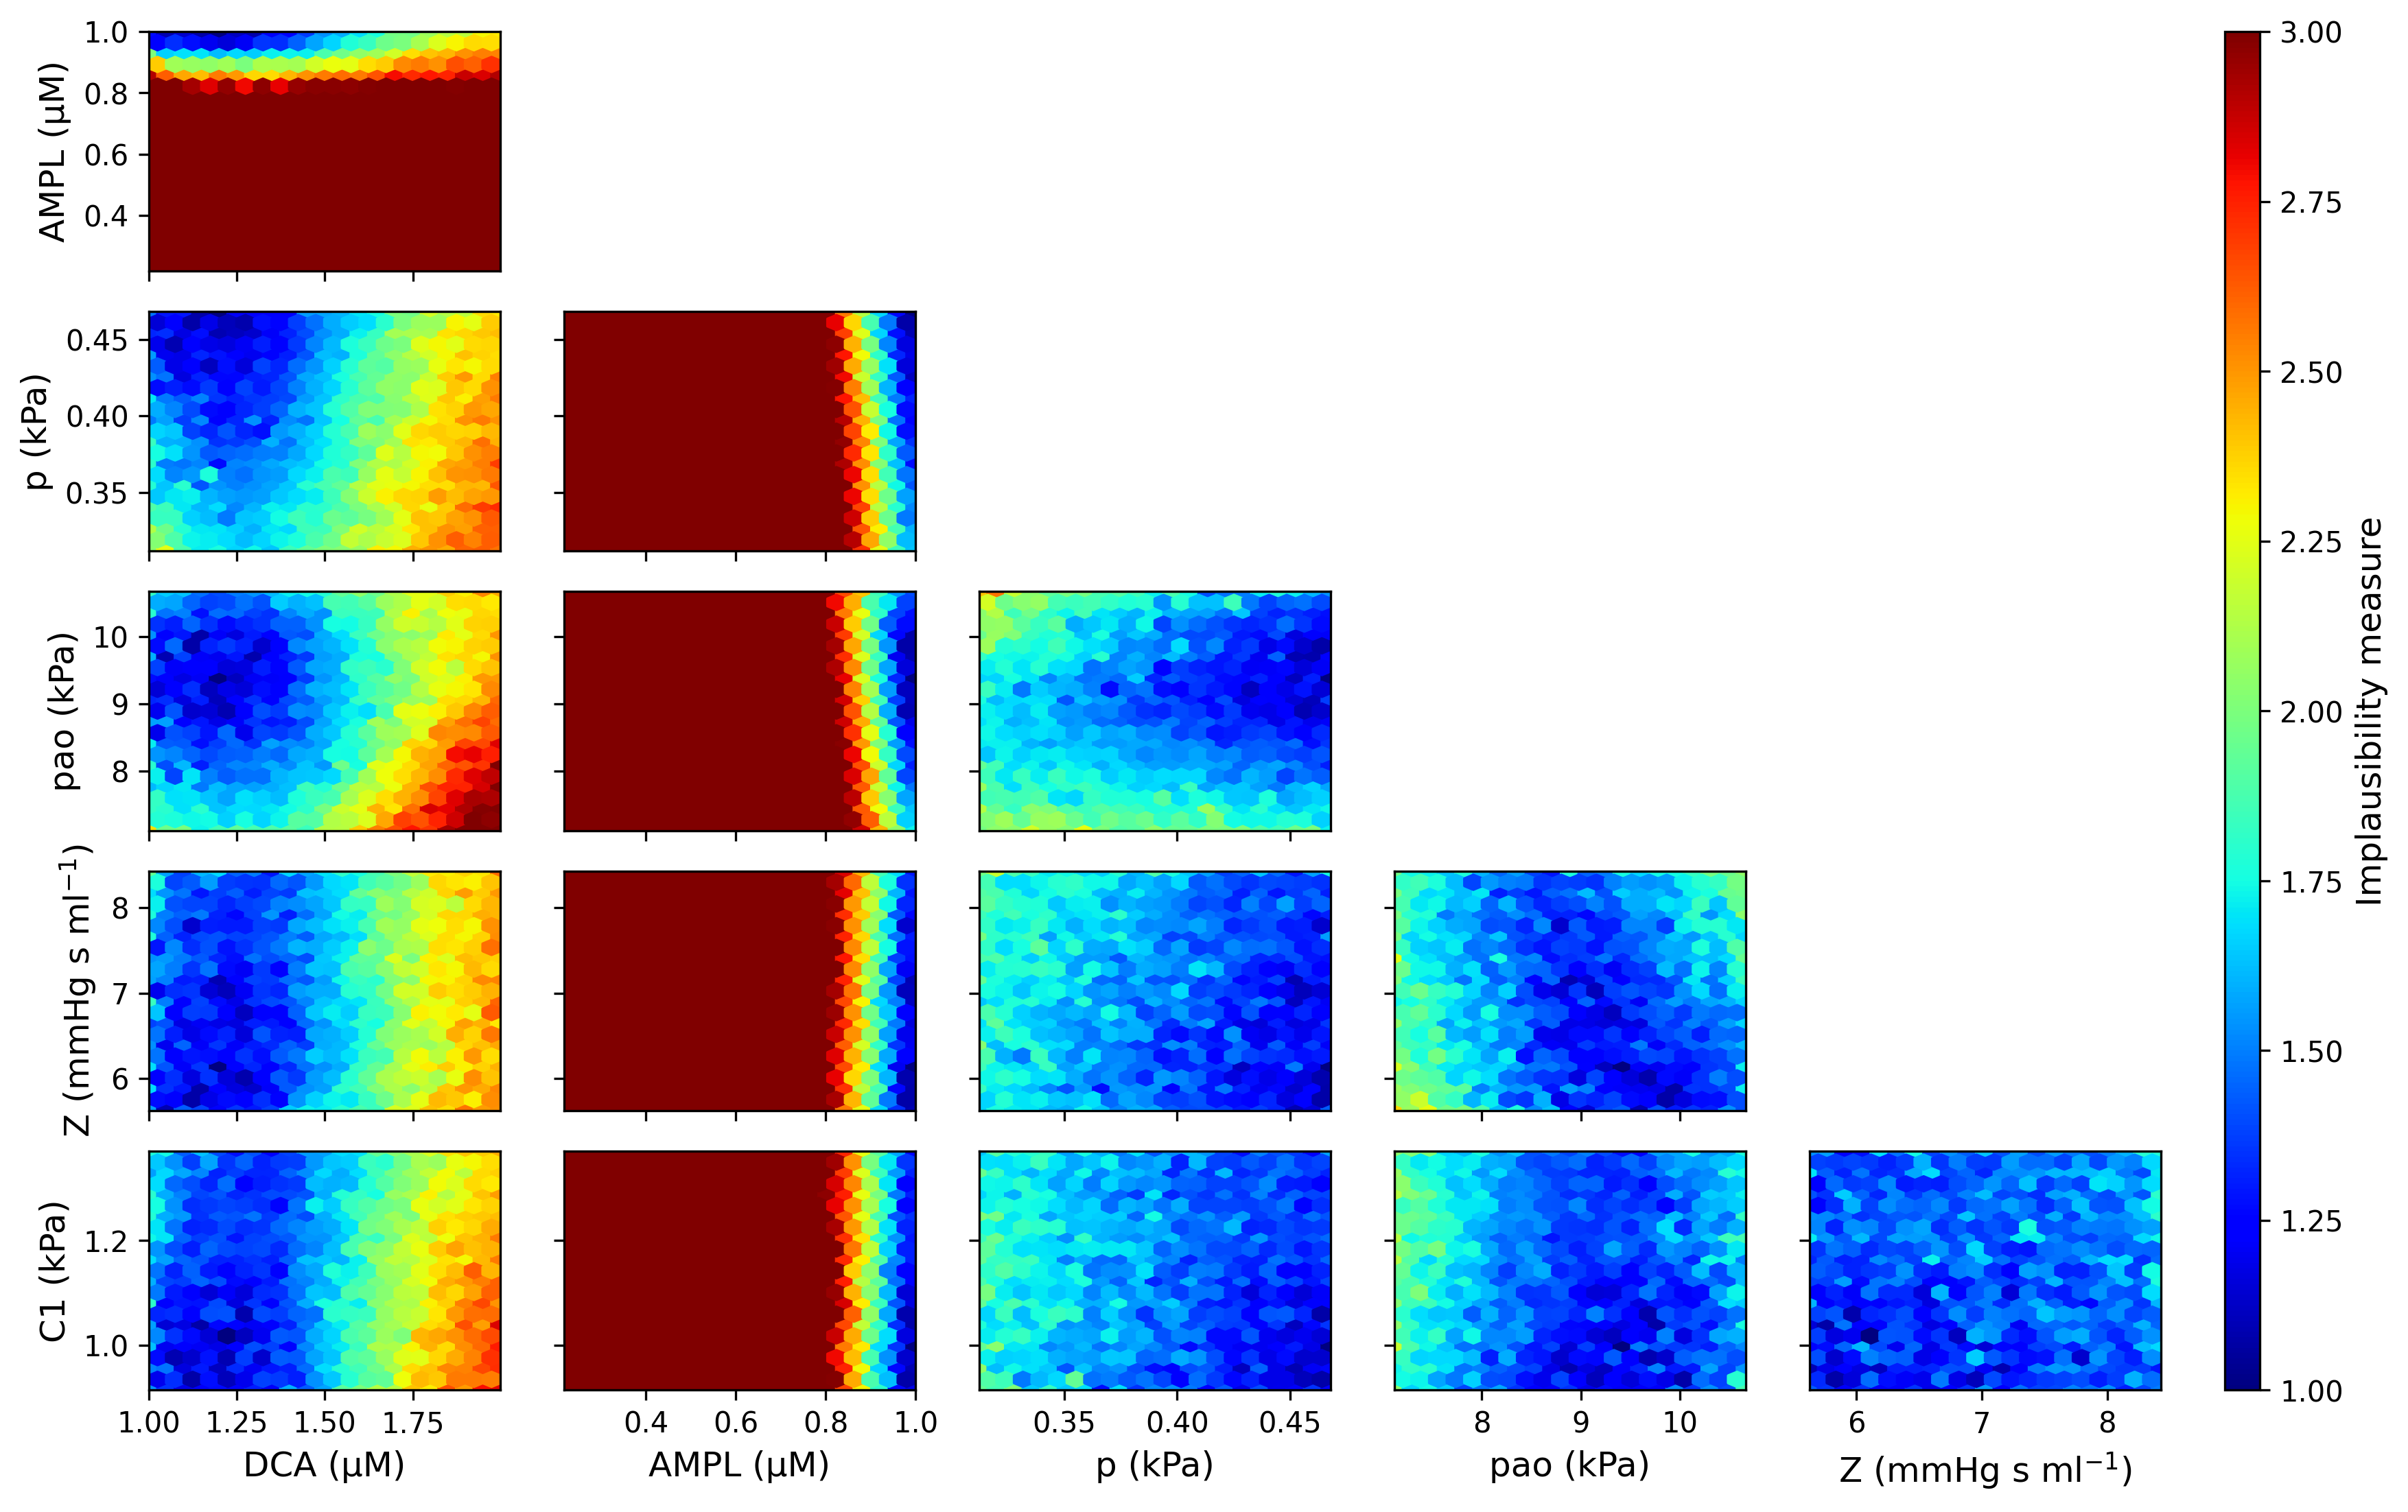
\includegraphics[width=\textwidth]{figures/chapter07/wave_1.png}
    \caption{First wave of history matching. The space represented by the parameters selected for optimisation is constrained according to an implausibility criterion which evaluates how plausible is a point to yield model predictions that are matching experimental observations.}  
    \label{fig:w1zsf1rat}
\end{figure}

\begin{figure}[ht!]
    \myfloatalign
    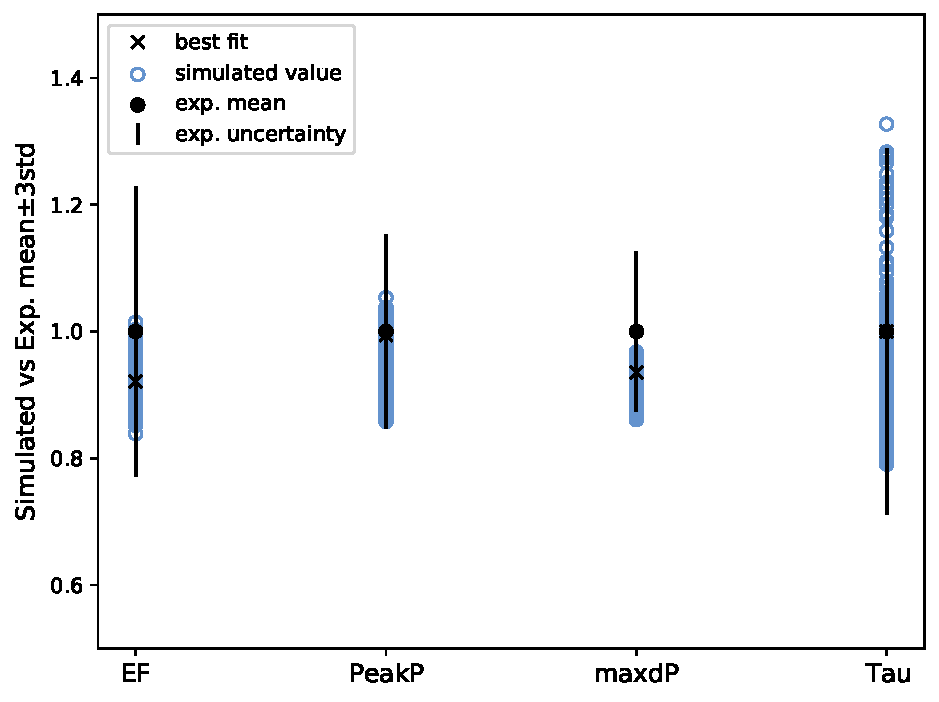
\includegraphics[width=0.6\textwidth]{figures/chapter07/w1_features_match.pdf}
    \caption{Matching experimental LV features' values. Simulator runs at input parameter points from the HM first (and also last) wave's non-implausible space. Obtained LV features’ (empty, blue dots) distributions around experimental mean values (filled, black dots) are all within 3 STD confidence intervals (vertical straight lines centred in their respective mean value). The best fit in weighted $L_1$ norm is also displayed (black cross). All the values including confidence intervals have been normalised by the respective experimental mean values.}
    \label{fig:w1bestzsf1model}
\end{figure}

\vspace{0.2cm}
In order to have a representative ZSF1 rat model to be used as a virtual platform for testing rat HFpEF-treating strategies, we selected one candidate represented by the best-fit according to a weighted $L_1$ norm where the last three LV features (PeakP, maxdP and Tau) which were shown to significantly change in the ZSF1 rat had double the weight of the first feature (EF) which showed no significant change, and with all the weights summing up to $1$. The obtained representative ZSF1 rat model $\Ca$ transient and PV loop are depicted in Figure~\ref{fig:shamandzsf1ratmodels}, and are compared with the reference SHAM rat model. The complete sets of re-fitted and fixed model parameters and corresponding LV features for both the reference, control SHAM rat model and the newly obtained, representative ZSF1 rat model are reported in Table~\ref{tab:bestfitparametersvalues} and Table~\ref{tab:bestfitfeaturesvalues}, respectively.

\begin{figure}[ht!]
    \myfloatalign
    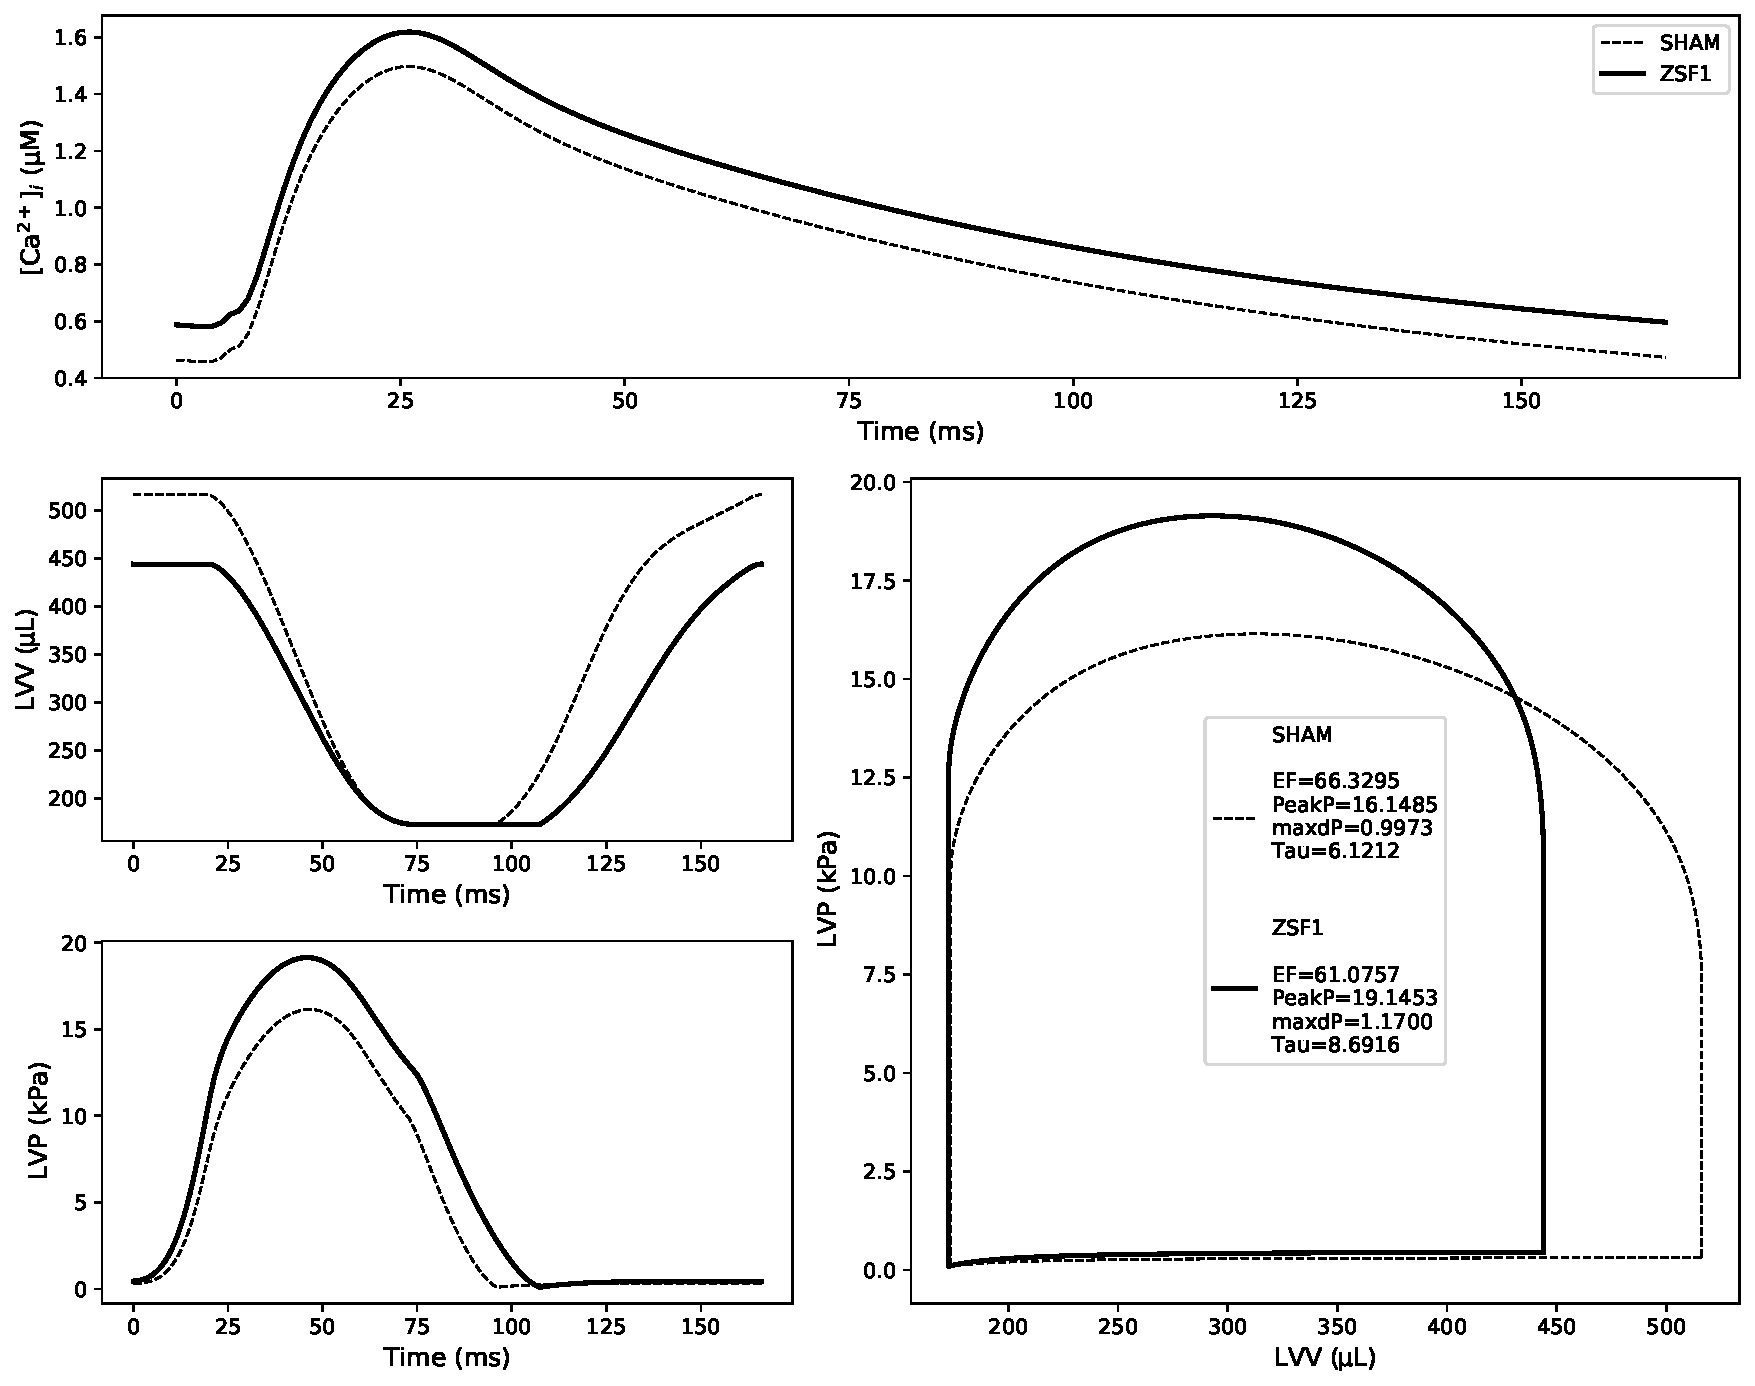
\includegraphics[width=\textwidth]{figures/chapter07/w1_resulting_bestfit_ca_and_pvloop.pdf}
    \caption{Representative SHAM and ZSF1 rat models calcium transients and pressure-volume loops. The ZSF1 rat model is created by perturbing the SHAM, healthy state. LV features which significantly changed from control to diseased animal are highlighted at the centre of the PV loops sub-plot. EF showed no significant change.}
    \label{fig:shamandzsf1ratmodels}
\end{figure}

\begin{table}[ht!]
    \myfloatalign
    \begin{tabularx}{\textwidth}{lXXX}
    \toprule
    \tableheadline{Parameter} & \tableheadline{Units} & \multicolumn{2}{c}{\spacedlowsmallcaps{Value}} \\
    \midrule
                              &                       & \tableheadline{SHAM} & \tableheadline{ZSF1} \\
    \midrule
    $\dca$                    & $\SI{}{\micro\Molar}$                 & $0.4632$      & $0.5870$ \\
    $\ampl$                   & $\SI{}{\micro\Molar}$                 & $1.0341$      & $1.0317$ \\
    $\tp$                     & $\SI{}{\milli\second}$                & $25.9474$     & $25.9474$ \\
    $\rtf$                    & $\SI{}{\milli\second}$                & $40.0807$     & $40.0807$ \\
    $\Caif$                   & $\SI{}{\micro\Molar}$                 & $2.1723$      & $2.1723$ \\
    $\beta_1$                 & $-$                                   & $-1.5$        & $-1.5$ \\
    $\koff$                   & $\SI{}{\per\milli\second}$            & $0.0515$      & $0.0515$ \\
    $\ntrpn$                  & $-$                                   & $2.0$         & $2.0$ \\
    $\kxb$                    & $\SI{}{\per\milli\second}$            & $0.0172$      & $0.0172$ \\
    $\nxb$                    & $-$                                   & $5.0$         & $5.0$ \\
    $\trpnf$                  & $-$                                   & $0.35$        & $0.35$ \\
    $\tref$                   & $\SI{}{\kilo\pascal}$                 & $156.067$     & $156.067$ \\
    $p$                       & $\SI{}{\kilo\pascal}$                 & $0.3122$      & $0.4481$ \\
    $\pao$                    & $\SI{}{\kilo\pascal}$                 & $7.1136$      & $10.3887$ \\
    $Z$                       & $\SI{}{\mmHg\second\per\milli\liter}$ & $5.6234$      & $7.4031$ \\
    $C_1$                     & $\SI{}{\kilo\pascal}$                 & $0.9141$      & $1.0670$ \\
    \bottomrule
    \end{tabularx}
    \caption{Representative SHAM and ZSF1 rat models' input parameters' values.}
    \label{tab:bestfitparametersvalues}
\end{table}

\begin{table}[ht!]
    \myfloatalign
    \begin{tabularx}{\textwidth}{lXXX}
    \toprule
    \tableheadline{LV feature} & \tableheadline{Units} & \multicolumn{2}{c}{\spacedlowsmallcaps{Value}} \\
    \midrule
                               &                       & \tableheadline{SHAM} & \tableheadline{ZSF1} \\
    \midrule
    $\textrm{EDV}$             & $\SI{}{\micro\liter}$                  & $516.23$      & $444.02$ \\
    $\textrm{ESV}$             & $\SI{}{\micro\liter}$                  & $173.82$      & $172.83$ \\
    $\textrm{SV}$              & $\SI{}{\micro\liter}$                  & $342.42$      & $271.19$ \\
    $\textrm{EF}$              & $\SI{}{\percent}$                      & $66.33$       & $61.08$ \\
    $\textrm{IVCT}$            & $\SI{}{\milli\second}$                 & $19.3$        & $19.7$ \\
    $\textrm{ET}$              & $\SI{}{\milli\second}$                 & $52.9$        & $54.6$ \\
    $\textrm{IVRT}$            & $\SI{}{\milli\second}$                 & $23.8$        & $33.0$ \\
    $\textrm{Tdiast}$          & $\SI{}{\milli\second}$                 & $93.5$        & $91.4$ \\
    $\textrm{PeakP}$           & $\SI{}{\kilo\pascal}$                  & $16.15$       & $19.15$ \\
    $\textrm{Tpeak}$           & $\SI{}{\milli\second}$                 & $46.6$        & $45.9$ \\
    $\textrm{ESP}$             & $\SI{}{\kilo\pascal}$                  & $10.04$       & $12.55$ \\
    $\textrm{maxdP}$ & $\SI{}{\kilo\pascal\per\milli\second}$           & $0.9973$      & $1.1700$ \\
    $\textrm{mindP}$ & $\SI{}{\kilo\pascal\per\milli\second}$           & $-0.5712$     & $-0.5276$ \\
    $\textrm{Tau}$                  & $\SI{}{\milli\second}$            & $6.1212$      & $8.6916$ \\
    \bottomrule
    \end{tabularx}
    \caption{Representative SHAM and ZSF1 rat models' output LV features' values.}
    \label{tab:bestfitfeaturesvalues}
\end{table}


%
%
%
\subsection{Recovered LV function in ZSF1 rats}\label{sec:ch7recovered_lv_function_in_zsf1_rats}
The new training datasets had dimensions of $104$, $129$, $114$ and $326$ points for the Ca, TNF, TKF and CaMYO groups, respectively. The GPEs' accuracy for each group are reported in Tables~\ref{tab:gpescores1}--\ref{tab:gpescores2}--\ref{tab:gpescores3}--\ref{tab:gpescores4}.

\begin{table}[ht!]
    \myfloatalign
    \begin{tabularx}{\textwidth}{XXX}
    \toprule
    \tableheadline{LV feature} & \tableheadline{$R^2$} & \tableheadline{$ISE_2 (\SI{}{\percent})$} \\
    \midrule
    $\textrm{EDV}$   & $\SI{0.9984}{}\pm\SI{0.0009}{}$ & $\SI{90.42}{}\pm\SI{6.70}{}$ \\
    $\textrm{ESV}$   & $\SI{0.9868}{}\pm\SI{0.0105}{}$ & $\SI{98.09}{}\pm\SI{3.80}{}$ \\
    $\textrm{PeakP}$ & $\SI{0.9940}{}\pm\SI{0.0045}{}$ & $\SI{93.33}{}\pm\SI{5.71}{}$ \\
    $\textrm{maxdP}$ & $\SI{0.9965}{}\pm\SI{0.0008}{}$ & $\SI{95.23}{}\pm\SI{4.25}{}$ \\
    $\textrm{Tau}$   & $\SI{0.9419}{}\pm\SI{0.0367}{}$ & $\SI{90.42}{}\pm\SI{6.70}{}$ \\
    \bottomrule
    \end{tabularx}
    \caption{GPEs' accuracy for the Ca parameter group.}
    \label{tab:gpescores1}
\end{table}

\begin{table}[ht!]
    \myfloatalign
    \begin{tabularx}{\textwidth}{XXX}
    \toprule
    \tableheadline{LV feature} & \tableheadline{$R^2$} & \tableheadline{$ISE_2 (\SI{}{\percent})$} \\
    \midrule
    $\textrm{EDV}$   & $\SI{0.9725}{}\pm\SI{0.0182}{}$ & $\SI{92.24}{}\pm\SI{4.86}{}$ \\
    $\textrm{ESV}$   & $\SI{0.9810}{}\pm\SI{0.0083}{}$ & $\SI{93.07}{}\pm\SI{5.65}{}$ \\
    $\textrm{PeakP}$ & $\SI{0.9557}{}\pm\SI{0.0235}{}$ & $\SI{89.93}{}\pm\SI{4.58}{}$ \\
    $\textrm{maxdP}$ & $\SI{0.9766}{}\pm\SI{0.0203}{}$ & $\SI{96.89}{}\pm\SI{2.88}{}$ \\
    $\textrm{Tau}$   & $\SI{0.9378}{}\pm\SI{0.0225}{}$ & $\SI{86.73}{}\pm\SI{11.97}{}$ \\
    \bottomrule
    \end{tabularx}
    \caption{GPEs' accuracy for the TNF parameter group.}
    \label{tab:gpescores2}
\end{table}

\begin{table}[ht!]
    \myfloatalign
    \begin{tabularx}{\textwidth}{XXX}
    \toprule
    \tableheadline{LV feature} & \tableheadline{$R^2$} & \tableheadline{$ISE_2 (\SI{}{\percent})$} \\
    \midrule
    $\textrm{EDV}$   & $\SI{0.9802}{}\pm\SI{0.0159}{}$ & $\SI{92.13}{}\pm\SI{6.36}{}$ \\
    $\textrm{ESV}$   & $\SI{0.9952}{}\pm\SI{0.0024}{}$ & $\SI{92.09}{}\pm\SI{7.49}{}$ \\
    $\textrm{PeakP}$ & $\SI{0.9937}{}\pm\SI{0.0020}{}$ & $\SI{92.13}{}\pm\SI{4.22}{}$ \\
    $\textrm{maxdP}$ & $\SI{0.9588}{}\pm\SI{0.0296}{}$ & $\SI{97.39}{}\pm\SI{3.47}{}$ \\
    $\textrm{Tau}$   & $\SI{0.8079}{}\pm\SI{0.1413}{}$ & $\SI{90.31}{}\pm\SI{7.53}{}$ \\
    \bottomrule
    \end{tabularx}
    \caption{GPEs' accuracy for the TKF parameter group.}
    \label{tab:gpescores3}
\end{table}

\begin{table}[ht!]
    \myfloatalign
    \begin{tabularx}{\textwidth}{XXX}
    \toprule
    \tableheadline{LV feature} & \tableheadline{$R^2$} & \tableheadline{$ISE_2 (\SI{}{\percent})$} \\
    \midrule
    $\textrm{EDV}$   & $\SI{0.9040}{}\pm\SI{0.0074}{}$ & $\SI{91.40}{}\pm\SI{4.42}{}$ \\
    $\textrm{ESV}$   & $\SI{0.6910}{}\pm\SI{0.0214}{}$ & $\SI{94.79}{}\pm\SI{1.81}{}$ \\
    $\textrm{PeakP}$ & $\SI{0.6986}{}\pm\SI{0.0639}{}$ & $\SI{94.47}{}\pm\SI{1.85}{}$ \\
    $\textrm{maxdP}$ & $\SI{0.9009}{}\pm\SI{0.0232}{}$ & $\SI{92.64}{}\pm\SI{3.54}{}$ \\
    $\textrm{Tau}$   & $\SI{0.7994}{}\pm\SI{0.0515}{}$ & $\SI{89.54}{}\pm\SI{4.72}{}$ \\
    \bottomrule
    \end{tabularx}
    \caption{GPEs' accuracy for the CaMYO parameter group.}
    \label{tab:gpescores4}
\end{table}

\vspace{0.2cm}
Information about performed waves, used cutoff values and percentages of space reduction are summarised in Table~\ref{tab:wavesprogress}. In Figure~\ref{fig:lvfeatsmatch} the HM waves progression is shown. For each LV feature we aimed to match, its values obtained when simulating parameter points from a specific wave's non-implausible region are plotted as a distribution, possibly overlapping to the experimental variability (red band) observed for the same feature. This is done at every wave run, so that the HM is represented as a sequence of LV features' values' distributions over consecutive waves.

\begin{table}[ht!]
    \myfloatalign
    \begin{tabularx}{\textwidth}{lXXXXXXXX}
    \toprule
    \tableheadline{Wave} & \multicolumn{8}{c}{\spacedlowsmallcaps{Parameter group}} \\
    \midrule
    & \multicolumn{2}{c}{\spacedlowsmallcaps{Ca}} & \multicolumn{2}{c}{\spacedlowsmallcaps{TNF}} & \multicolumn{2}{c}{\spacedlowsmallcaps{TKF}} & \multicolumn{2}{c}{\spacedlowsmallcaps{CaMYO}} \\
    \midrule
    & $I_{\,\textrm{cutoff}}$ & NIMP ($\SI{}{\percent}$) & $I_{\,\textrm{cutoff}}$ & NIMP ($\SI{}{\percent}$) & $I_{\,\textrm{cutoff}}$ & NIMP ($\SI{}{\percent}$) & $I_{\,\textrm{cutoff}}$ & NIMP ($\SI{}{\percent}$) \\ 
    \midrule
    $1$ & $4.5$ & $0.08$ & $4.0$ & $0.01$ & $4.0$ & $0.07$ & $4.0$ & $13.75$ \\
    $2$ & $4.5$ & $0.18$ & $4.0$ & $0.33$ & $4.0$ & $0.14$ & $4.0$ & $73.78$ \\
    $3$ & $4.2$ & $6.53$ & $4.0$ & $0.80$ & $-$ & $-$  & $3.5$ & $55.03$ \\
    $4$ & $4.2$ & $92.79$  & $-$ & $-$  & $-$ & $-$  & $3.5$ & $84.39$ \\
    $5$ & $-$ & $-$  & $-$ & $-$  & $-$ & $-$  & $3.0$ & $55.98$ \\
    $6$ & $-$ & $-$  & $-$ & $-$  & $-$ & $-$  & $3.0$ & $84.43$ \\
    $7$ & $-$ & $-$  & $-$ & $-$  & $-$ & $-$  & $2.5$ & $47.94$ \\
    $8$ & $-$ & $-$  & $-$ & $-$  & $-$ & $-$  & $2.5$ & $83.97$ \\
    $9$ & $-$ & $-$  & $-$ & $-$  & $-$ & $-$  & $2.0$ & $34.12$ \\
    $10$ & $-$ & $-$  & $-$ & $-$  & $-$ & $-$  & $2.0$ & $75.03$ \\
    \bottomrule
    \end{tabularx}
    \caption{Details of history matching progression. HM is run for each parameter group in order to re-fit the specific parameters within the group. Parameter points ($400,000$ at Wave $1$ and $100,000$ at the next Waves) are tested against an implausibility criterion using the reported cutoff values, and only a percentage of these points resulted to be non-implausible (NIMP).}
    \label{tab:wavesprogress}
\end{table}

\begin{figure}[ht!]
    \myfloatalign
    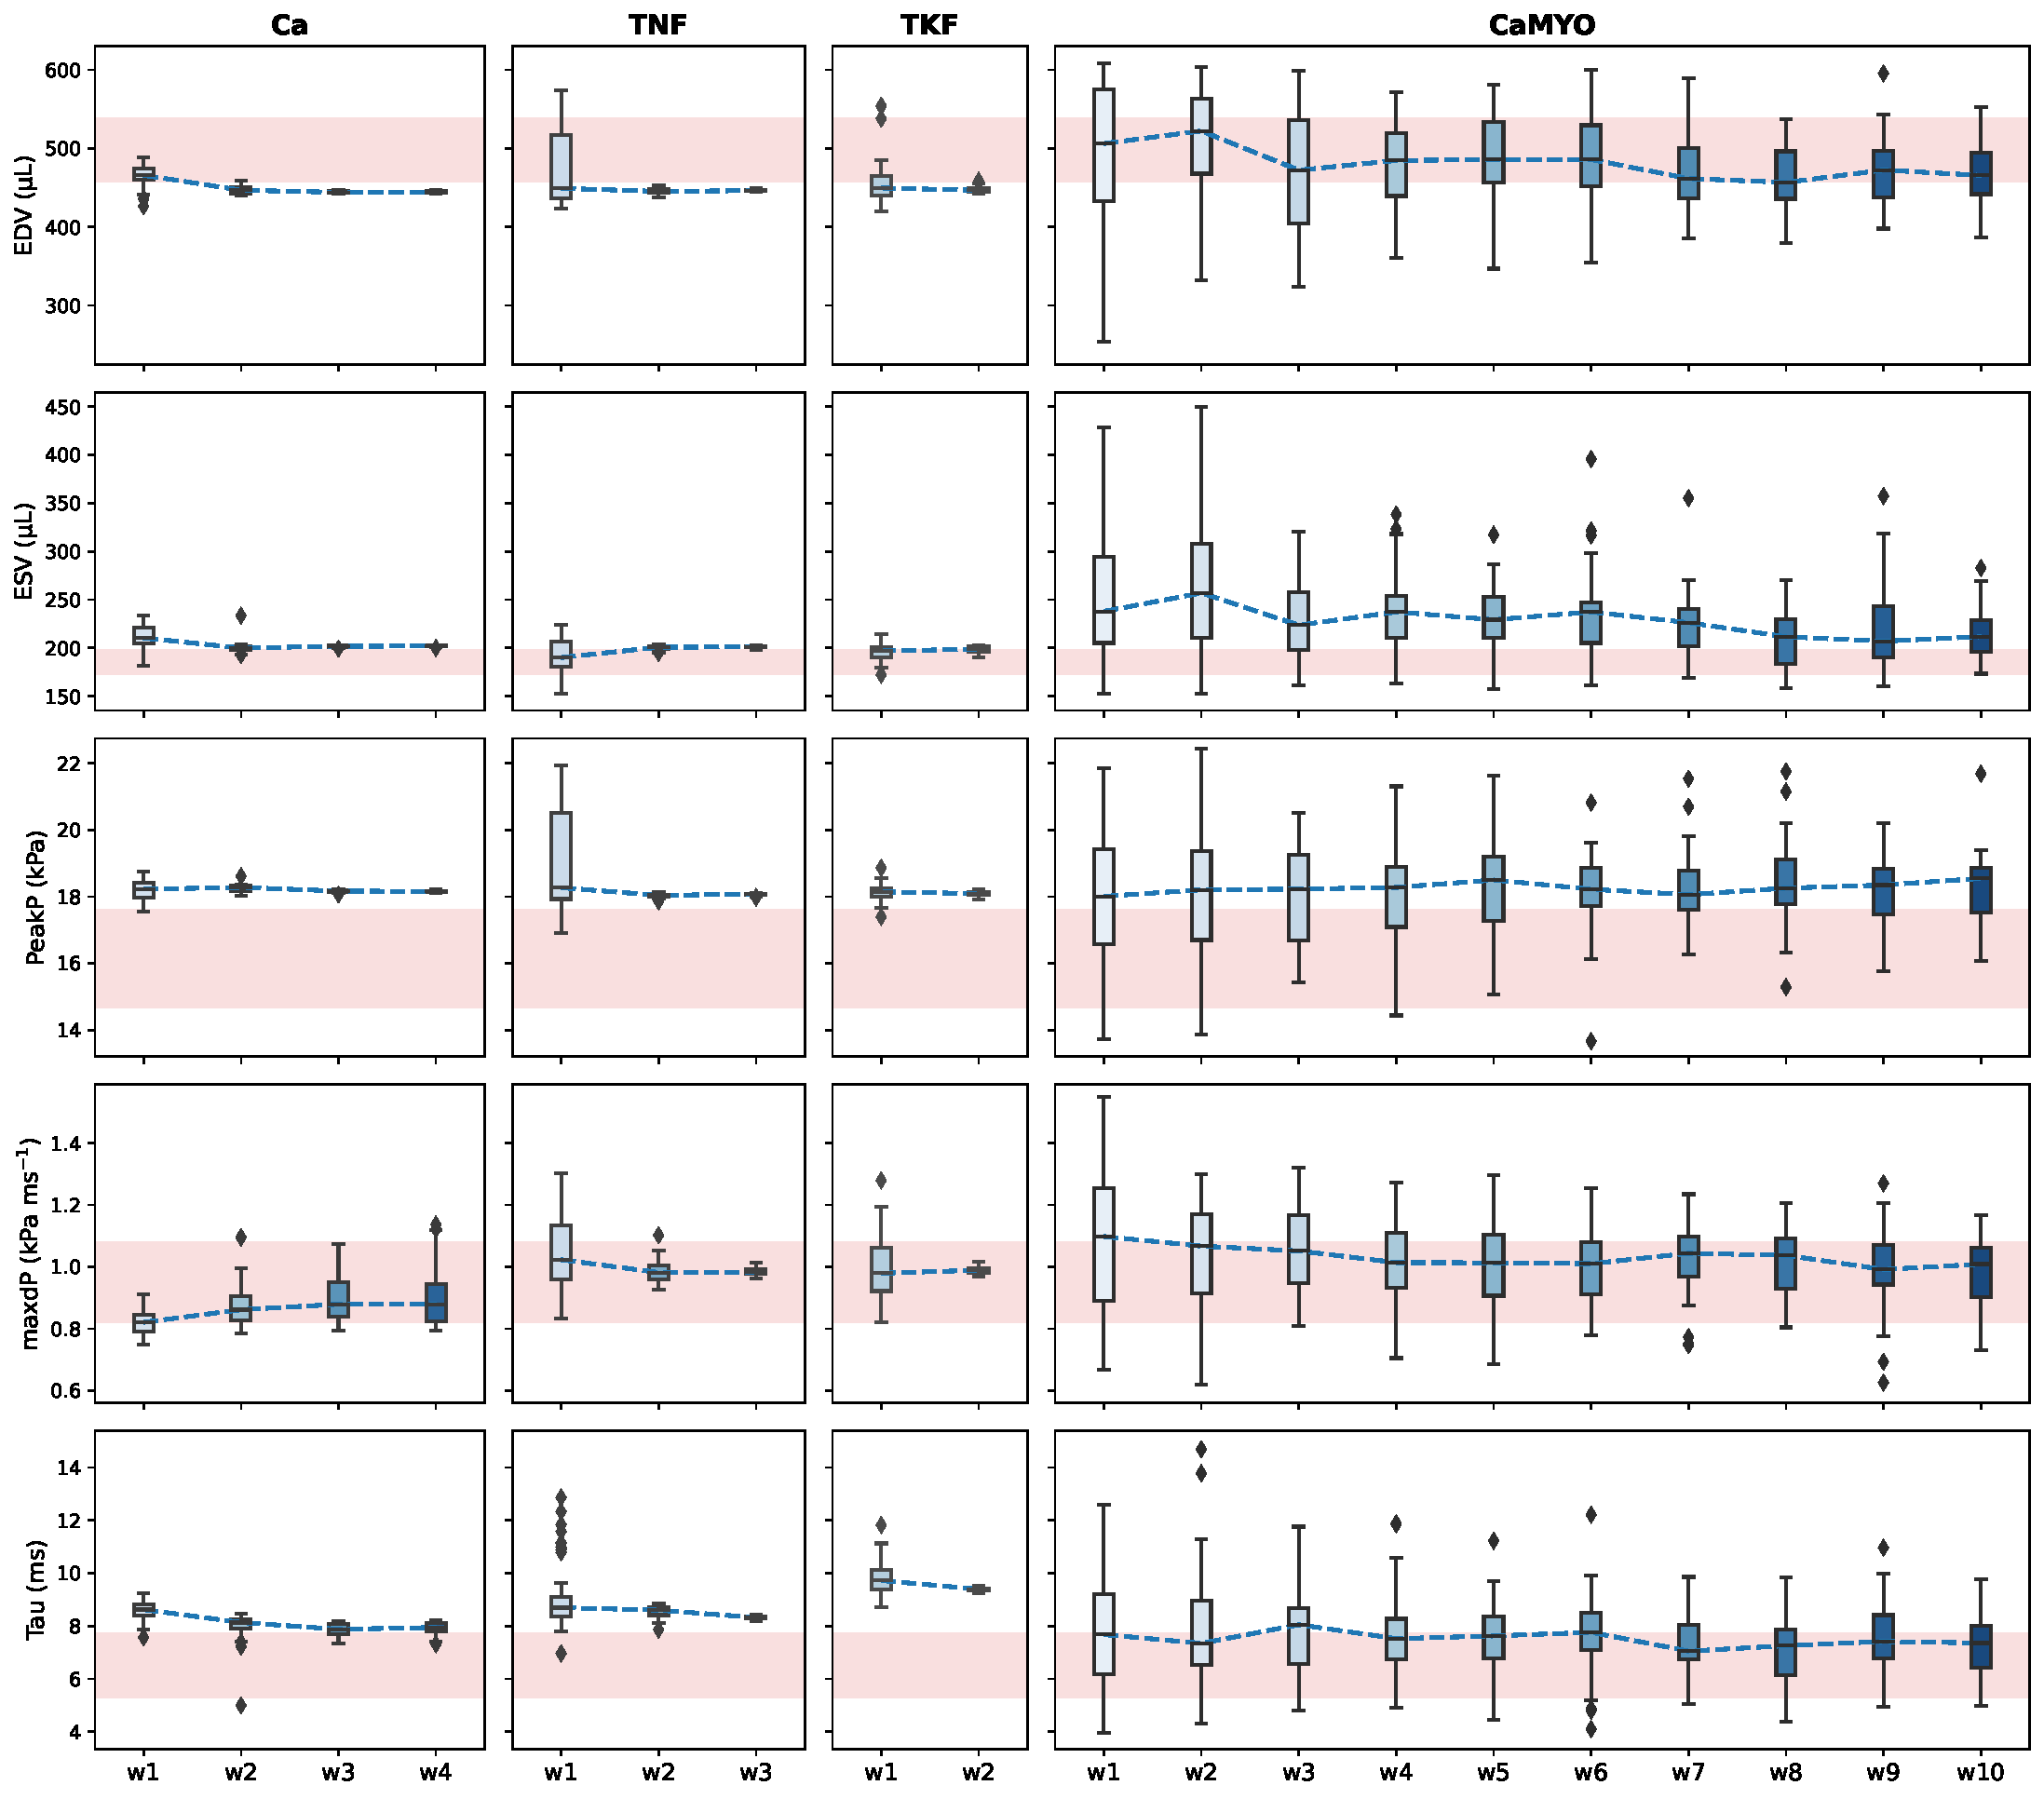
\includegraphics[width=\textwidth]{figures/chapter07/Fig_6.pdf}
    \caption{History matching waves progression. At each wave, $128$ points are simulated from the current non-implausible parameter region and the features' values from the converging simulations are plotted as box plots coloured in blue variants for different consecutive waves. The median trend of these distributions is represented by a dashed blue line. Mean $\pm\,3$ standard deviations target intervals are represented in light red-coloured shaded areas for each LV feature.}
    \label{fig:lvfeatsmatch}
\end{figure}

\vspace{0.2cm}
For each parameter group, we can distinguish whether a specific LV feature has been recovered by looking at the last wave' distribution. Specifically, a feature was determined to be recovered if this distribution median was within the uncertainty region for that feature. We can see that we were able to recover the $\textrm{maxdP}$ feature in all $4$ cases. $\textrm{EDV}$ and $\textrm{Tau}$ features were only recovered in the CaMYO group. $\textrm{ESV}$ feature was harder to recover, being very close to the uncertainty region in all the $4$ cases although never meeting the median-based criterion. $\textrm{PeakP}$ was never recovered, although it moved in the correct direction of recovery (decreasing) in all $4$ cases. For each group, we selected (according to an $L_2$-norm best-fit criterion) a reference recovered rat model which we labelled as ``RECOV", and we plotted the respective LV pressure and volume transients and PV loops (Figure~\ref{fig:bestfits}), compared with the reference SHAM rat and ZSF1 rat models.

\begin{figure}[ht!]
    \myfloatalign
    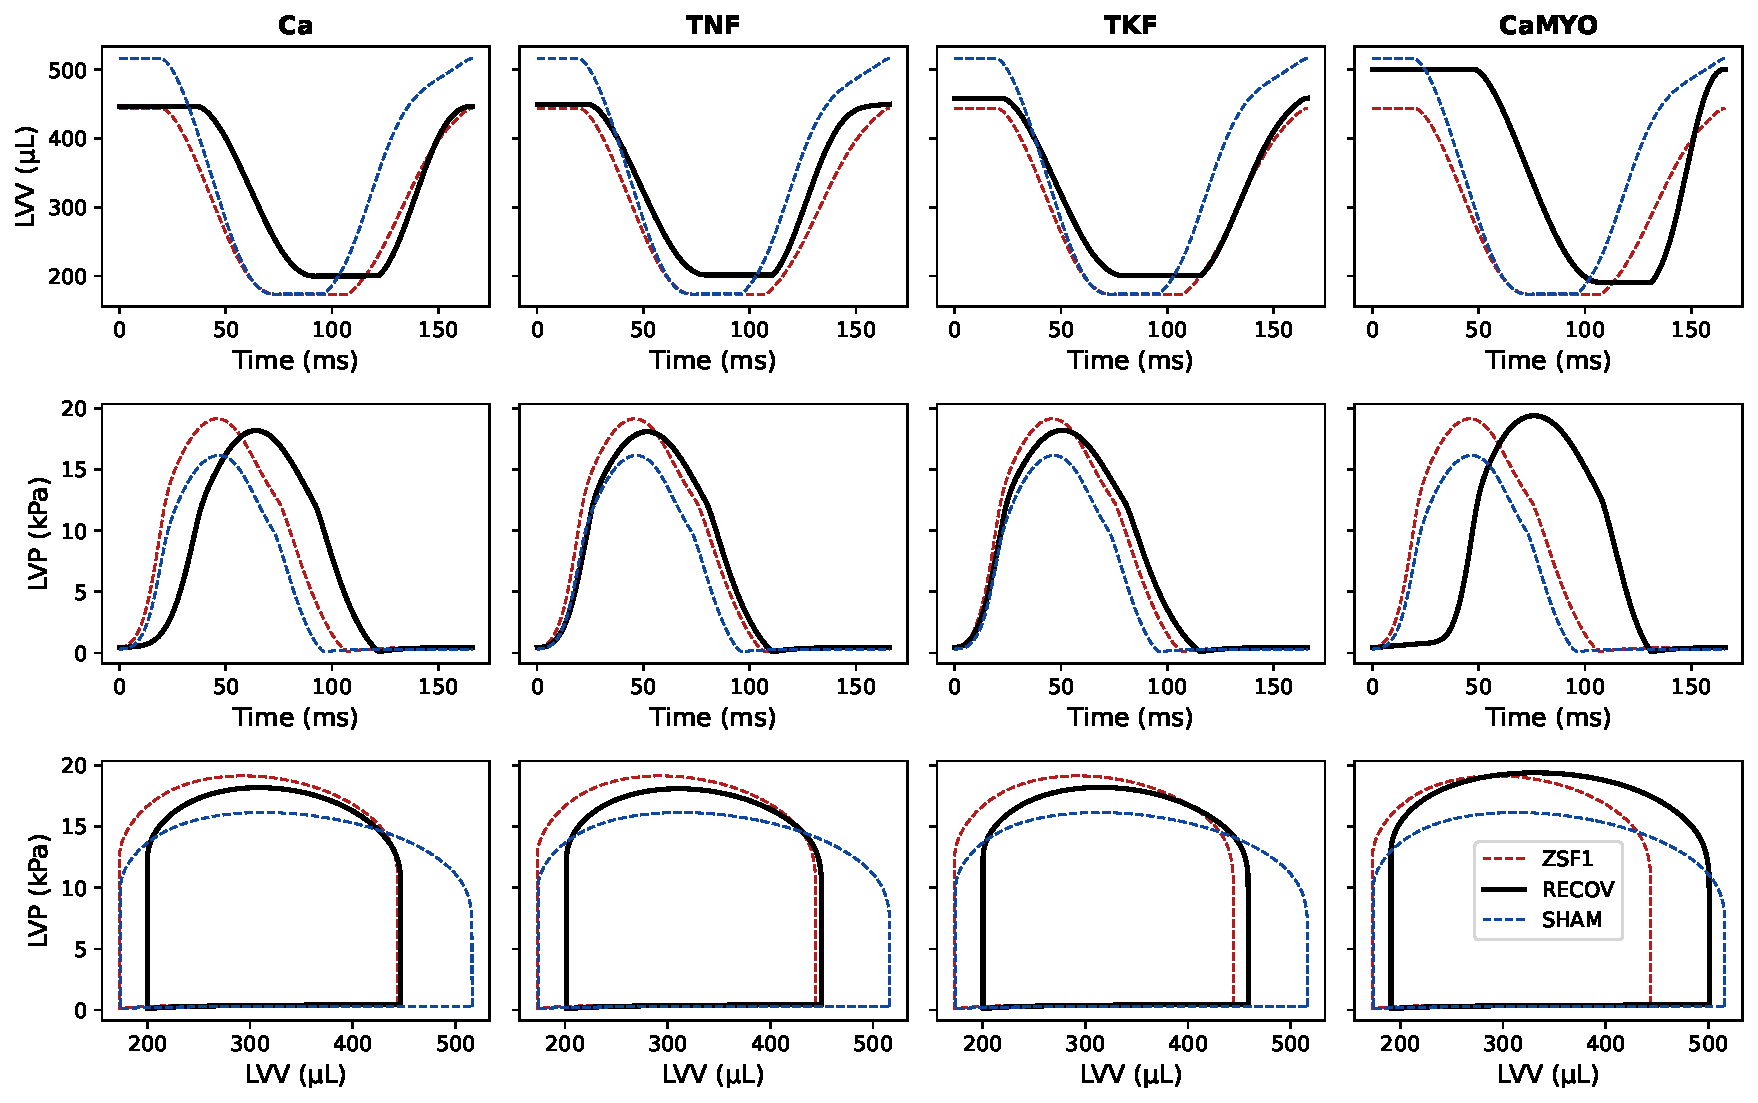
\includegraphics[width=\textwidth]{figures/chapter07/Fig_7.pdf}
    \caption{Best fit recovered rat heart models. For each parameter group, the last wave fitted models are compared against the target mean which the history matching aimed to match, and the best-fit model is selected according to the $L_2$-norm. This best-fit rat model (RECOV, black thick line) is compared with the reference ZSF1 rat model (red dashed line) and with the reference SHAM rat model (blue dashed line).}
    \label{fig:bestfits}
\end{figure}

\vspace{0.2cm}
By relaxing the median-based recovery criterion, we also looked at whether the last wave' distribution of a specific LV feature $i$ had a median value $y_{i}^{\textrm{RECOV}}$ which was moving towards the healthy experimental mean value $y_{i}^{\textrm{SHAM}}$ starting from the reference, diseased state value $y_{i}^{\textrm{ZSF1}}$. For each parameter group, we computed the percentage of recovery $R_{\textrm{perc}}$ for each LV feature as described by the ratio:
%
\begin{equation}
    R_{\textrm{perc}} = \left|\frac{y_{i}^{\textrm{RECOV}}-y_{i}^{\textrm{ZSF1}}}{y_{i}^{\textrm{SHAM}}-y_{i}^{\textrm{ZSF1}}}\right|
\end{equation}

\vspace{0.2cm}\noindent
A value of $R_{\textrm{perc}}=1$ indicates that the feature has been recovered fully. When the median of a given LV feature's distribution was not moving towards the correct direction of recovery, its corresponding $R_{\textrm{perc}}$ value was set to $0$. When the median was moving towards the correct direction of recovery but surpassed the healthy value, its corresponding $R_{\textrm{perc}}$ value was set to $1$ instead. $R_{\textrm{perc}}$ values for each LV feature for each group are summarised in Table~\ref{tab:percrecov}. We can see that the highest degree of recovery ($\SI{39}{\percent}$) can be achieved when manipulating both the sarcomere kinetics and the $\Ca$ dynamics at the same time. It is worth noticing that the different degrees of recovery achieved by targeting the first three groups of parameters, namely $\SI{34}{\percent}$, $\SI{28}{\percent}$ and $\SI{24}{\percent}$ for Ca, TNF and TKF groups, respectively, match the relative importance these groups have into explaining the total variance of the considered LV features (Table~\ref{tab:paramsranking}).

\begin{table}[ht!]
    \myfloatalign
    \begin{tabularx}{\textwidth}{lXXXX}
    \toprule
    \tableheadline{LV feature}    & \multicolumn{4}{c}{\spacedlowsmallcaps{Parameter group}} \\ \midrule
                        & Ca & TNF & TKF & CaMYO \\ \midrule
    $\textrm{EDV}$      & $0.01$ & $0.04$ & $0.05$ & $0.40$ \\
    $\textrm{ESV}$      & $0.00$ & $0.00$ & $0.00$ & $0.00$ \\
    $\textrm{PeakP}$    & $0.33$ & $0.36$ & $0.35$ & $0.20$ \\
    $\textrm{maxdP}$    & $1.00$ & $0.85$ & $0.82$ & $0.73$ \\
    $\textrm{Tau}$      & $0.34$ & $0.17$ & $0.00$ & $0.61$ \\ \midrule
    \textbf{Mean recovery} & $0.34$ & $0.28$ & $0.24$ & $0.39$ \\
    \bottomrule
    \end{tabularx}
    \caption{LV features' percentages of recovery. For each LV feature we aimed to recover, the distance between its median recovered value and the respective healthy value is divided by the distance between the initial, diseased value and the healthy value. This ratio describes the percentage of recovery for the examined feature.}
    \label{tab:percrecov}
\end{table}

\vspace{0.2cm}
We further inspected the parameter space which the HM converged to in the last wave for each parameter group, and we compared this with the ZSF1 rat model reference parameter set (see Figure~\ref{fig:paramsdistr}). The distribution's median trend over consecutive waves of each parameter within each group provides indication on which direction the parameter has undergone a perturbation from the reference ZSF1 rat same parameter value in order to recover the LV function. This is summarised in Table~\ref{tab:virtualdrugeffects} for the last waves' perturbations.

\begin{figure}[ht!]
    \myfloatalign
    \subfloat[Ca parameter group]{
    \label{fig:paramsdistr1}
    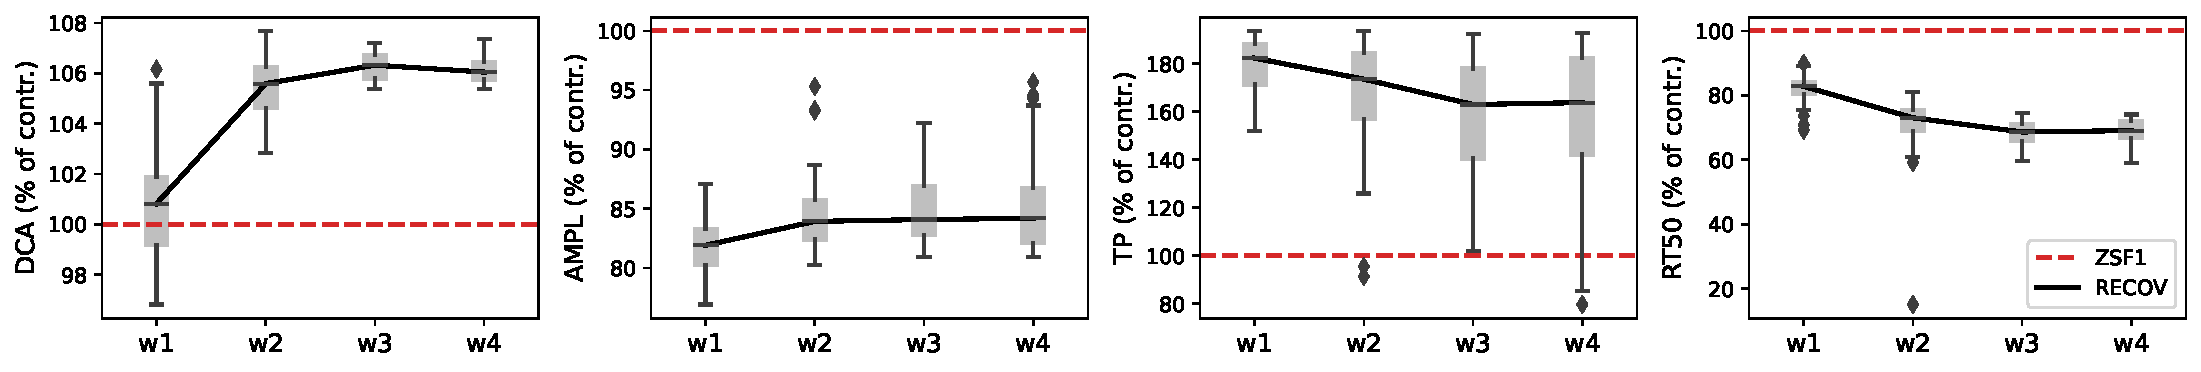
\includegraphics[width=\textwidth]{figures/chapter07/Fig_8a.pdf}}\quad
    \subfloat[TNF parameter group]{
    \label{fig:paramsdistr2}
    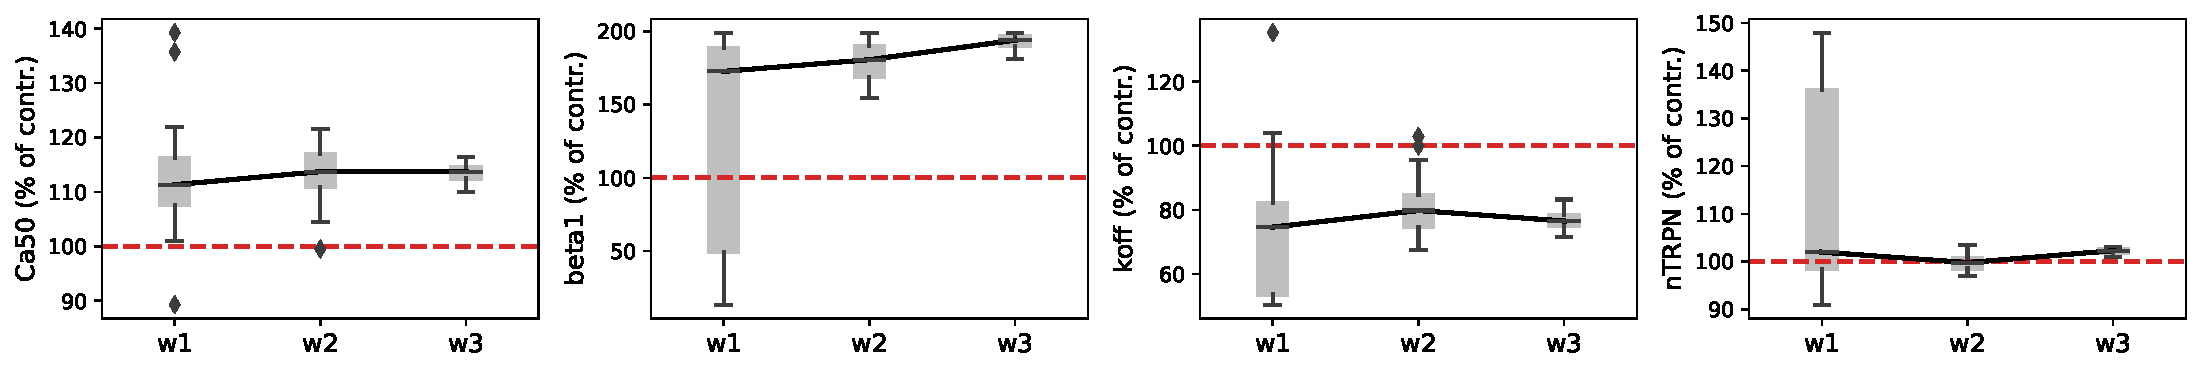
\includegraphics[width=\textwidth]{figures/chapter07/Fig_8b.pdf}}\quad
    \subfloat[TKF parameter group]{
    \label{fig:paramsdistr3}
    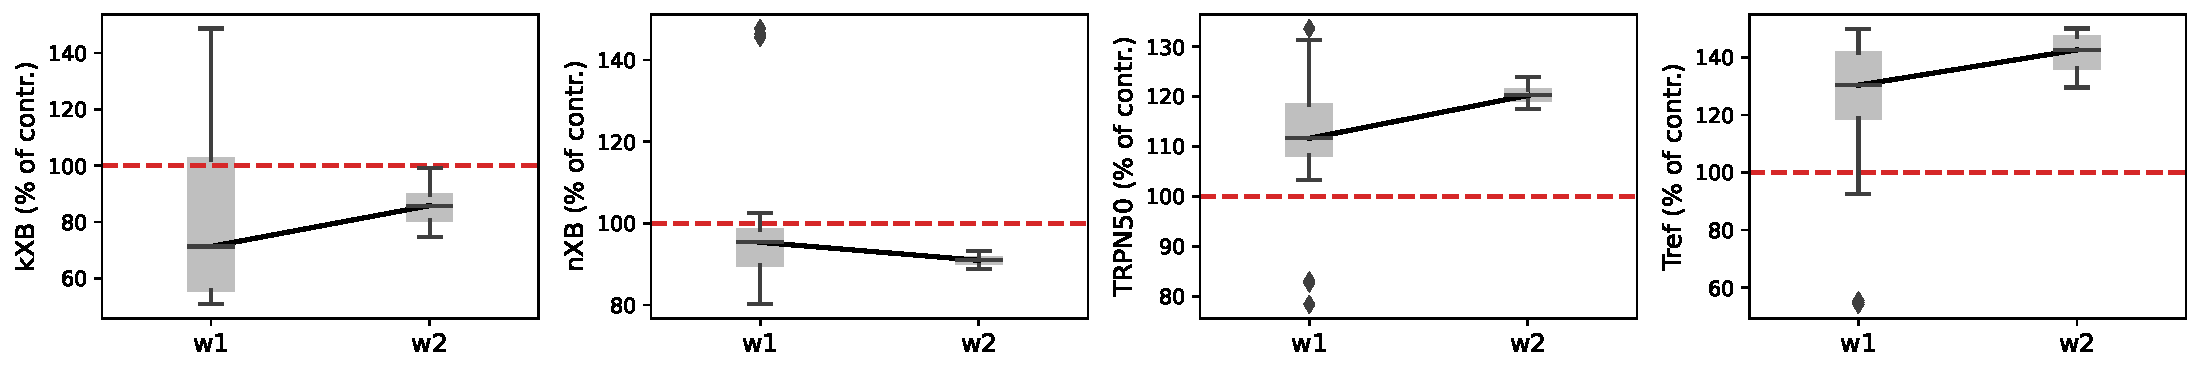
\includegraphics[width=\textwidth]{figures/chapter07/Fig_8c.pdf}}\quad
    \subfloat[CaMYO parameter group]{
    \label{fig:paramsdistr4}
    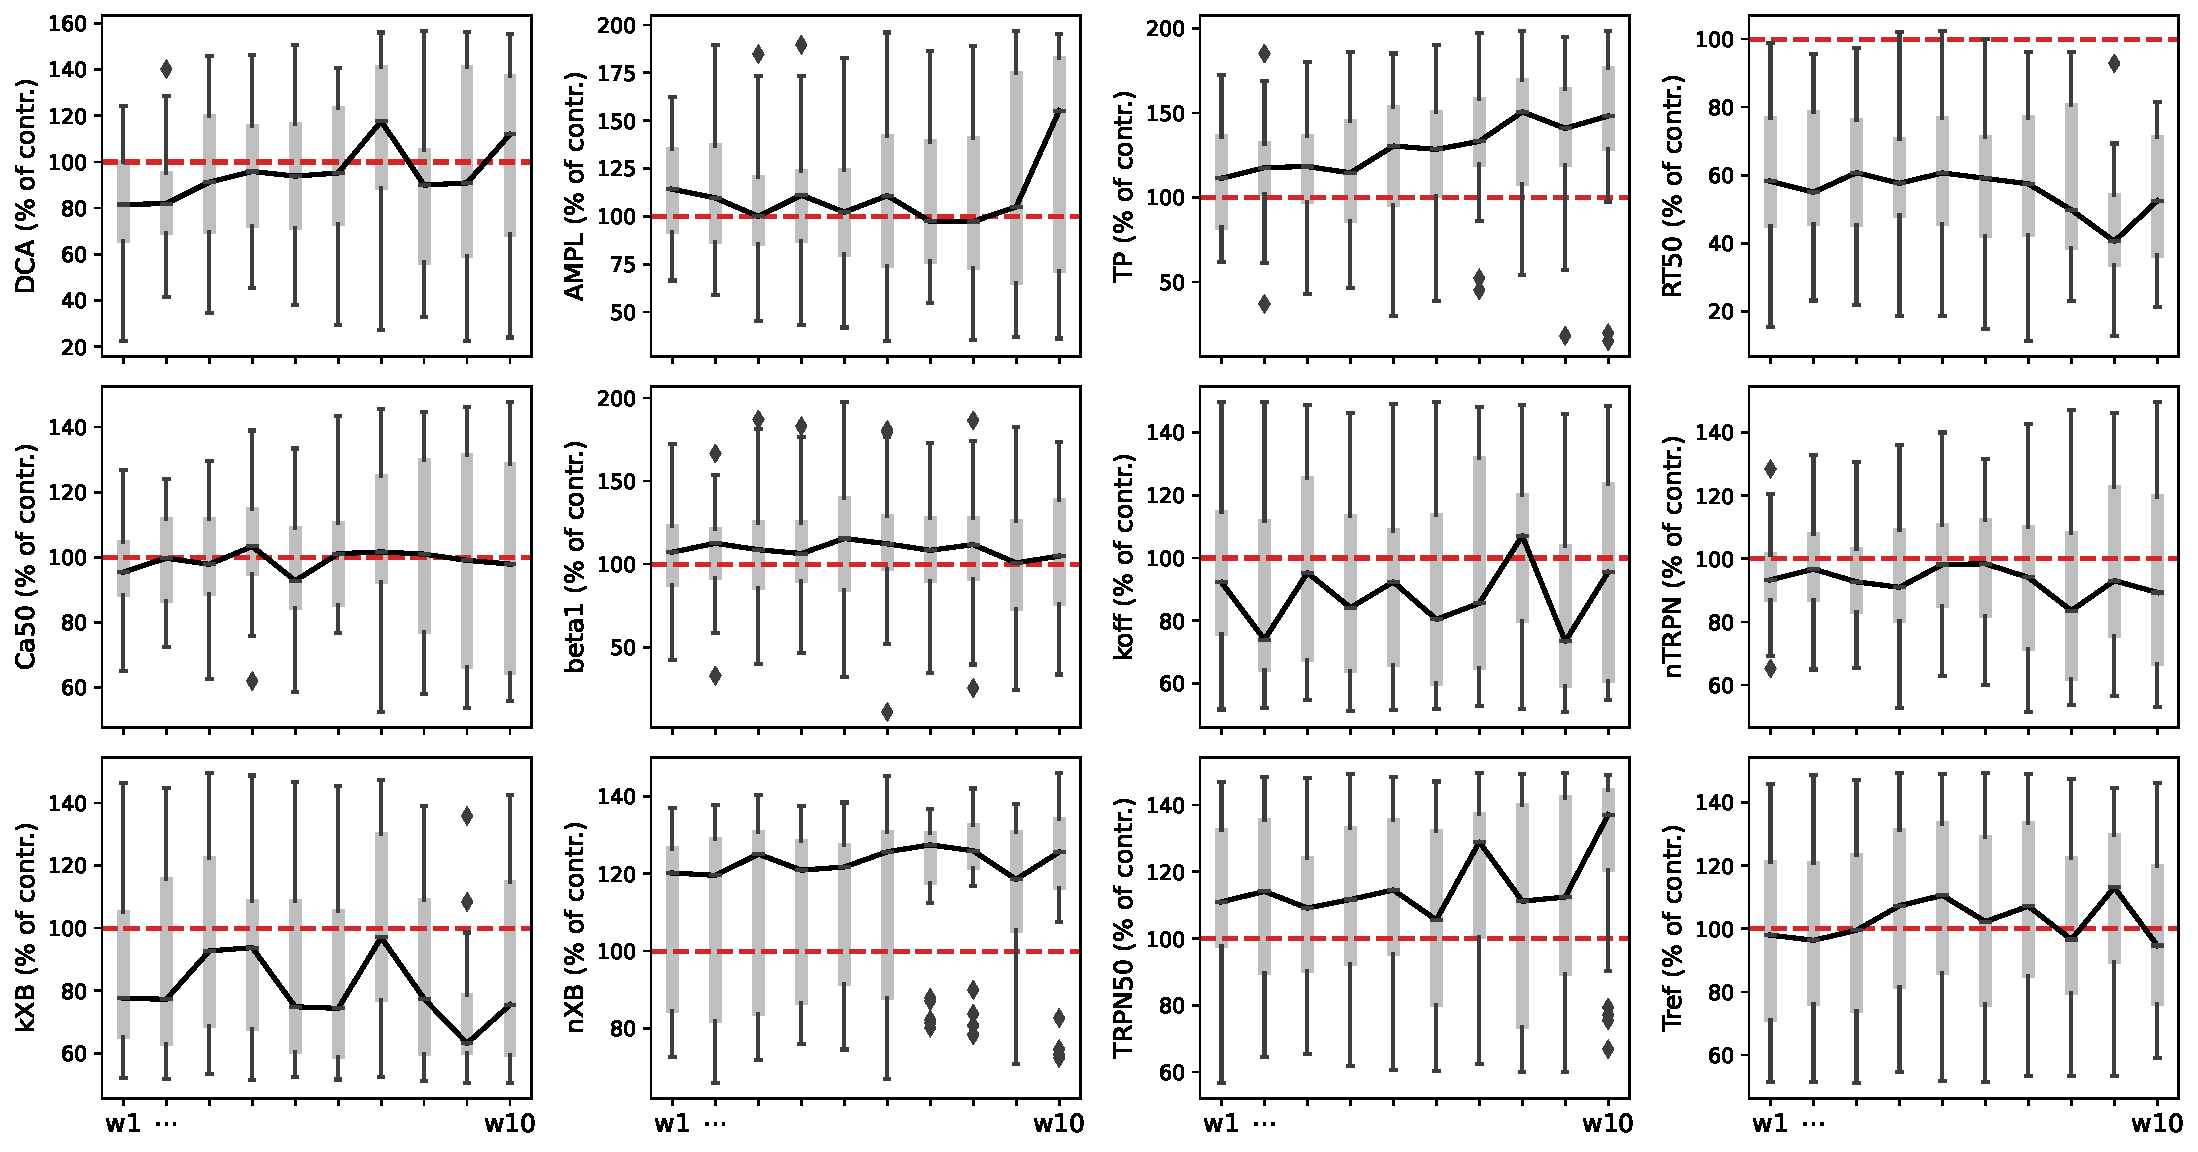
\includegraphics[width=\textwidth]{figures/chapter07/Fig_8d.pdf}}
    \caption{Parameter distributions across progressing waves for the four different parameter groups. Each parameter distribution is represented as a grey box plot at each wave. Its median trend during multiple waves is highlighted in a solid black line and is compared with the ZSF1 rat model reference value for the same parameter highlighted in a dashed red line. All the plotted RECOV parameter values are given as percentages of the respective baseline ZSF1 parameter values.}
    \label{fig:paramsdistr}
\end{figure}

\begin{table}[ht!]
    \myfloatalign
    \begin{tabularx}{\textwidth}{lXXXX}
    \toprule
    \tableheadline{Group} & \tableheadline{Parameter} & \tableheadline{ZSF1} & \tableheadline{RECOV} & \tableheadline{Change ($\SI{}{\percent}$)} \\
    \midrule
    \multirow{4}{*}{Ca} & $\dca$ & $1.2674$ & $1.3440$ & $6.05$ \\
    & $\ampl$ & $0.9977$ & $0.8399$ & $-15.82$ \\
    & $\tp$ & $1.0000$ & $1.6379$ & $63.79$ \\
    & $\rtf$ & $1.0000$ & $0.6906$ & $-30.95$ \\
    \midrule
    \multirow{4}{*}{TNF} & $\Caif$ & $2.1723$ & $2.4699$ & $13.70$ \\
    & $\betaone$ & $-1.50$ & $-2.91$ & $-93.91$ \\
    & $\koff$ & $0.0515$ & $0.0394$ & $-23.47$ \\
    & $\ntrpn$ & $2.00$ & $2.05$ & $2.28$ \\
    \midrule
    \multirow{4}{*}{TKF} & $\kxb$ & $0.0172$ & $0.0147$ & $-14.18$ \\
    & $\nxb$ & $5.00$ & $4.55$ & $-9.07$ \\
    & $\trpnf$ & $0.35$ & $0.42$ & $20.24$ \\
    & $\tref$ & $156.067$ & $222.420$ & $42.52$ \\
    \midrule
    \multirow{12}{*}{CaMYO} & $\dca$ & $1.2674$ & $1.4200$ & $12.04$ \\
    & $\ampl$ & $0.9977$ & $1.5486$ & $55.22$ \\
    & $\tp$ & $1.0000$ & $1.4828$ & $48.28$ \\
    & $\rtf$ & $1.0000$ & $0.5247$ & $-47.53$ \\
    & $\Caif$ & $2.1723$ & $2.1268$ & $-2.10$ \\
    & $\betaone$ & $-1.50$ & $-1.57$ & $-4.86$ \\
    & $\koff$ & $0.0515$ & $0.0492$ & $-4.44$ \\
    & $\ntrpn$ & $2.00$ & $1.79$ & $-10.69$ \\
    & $\kxb$ & $0.0172$ & $0.0130$ & $-24.44$ \\
    & $\nxb$ & $5.00$ & $6.28$ & $25.61$ \\
    & $\trpnf$ & $0.35$ & $0.48$ & $37.12$ \\
    & $\tref$ & $156.067$ & $147.785$ & $-5.31$ \\
    \bottomrule
    \end{tabularx}
    \caption{Percentage perturbations of cardiac cellular properties resulting from the last waves' parameter spaces. For each parameter last wave distribution, its median value is given as a $\pm$ percentage perturbation from the corresponding ZSF1 reference value. $\Ca$ transient parameters are reported as coefficients used to scale the corresponding SHAM rat baseline real parameter values.}
    \label{tab:virtualdrugeffects}
\end{table}

\vspace{0.2cm}
We can see that in order to recover the LV function by only perturbing the $\Ca$ transient ($4$ parameters), $\dca$ and $\tp$ increased, while $\ampl$ and $\rtf$ decreased. This resulted in a $\Ca$ transient signal which was shifted upwards, flatter and delayed in time with fast recovery. By only perturbing the thin filament properties ($4$ parameters), the LV function could be recovered when $\Caif$ increased at a constant $\ntrpn$, with decreased $\betaone$ and $\koff$. This resulted in TnC-$\Ca$ bound complexes saturating at lower $\Cai$ and to a slower dissociation of the TnC-$\Ca$ bound state which in turns made actin binding sites available for longer. By only perturbing the thick filament properties ($4$ parameters), the LV function could be recovered when $\nxb$ and $\kxb$ decreased with increased $\trpnf$ and $\tref$. This resulted in an overall slower force generation with increased maximal generated force. Lastly, when manipulating both the $\Ca$ transient and the whole sarcomere at the same time ($12$ parameters) to recover the LV function, $\ampl$ and $\tp$ were increased at a constant $\dca$ and decreased $\rtf$; $\koff$ and $\ntrpn$ were decreased at a constant $\Caif$ and $\betaone$; $\nxb$ and $\trpnf$ were increased at a constant $\tref$ and decreased $\kxb$.

\vspace{0.2cm}
To interpret these changes in terms of intact muscle experimental measurements, we used the contraction model~\cite{Land:2012*a} to estimate the corresponding changes in steady state force-calcium relationship and field stimulated isometric tension transient predicted by the model to recover cardiac function in the ZSF1 model. This is illustrated in Figure~\ref{fig:fpcatension}. Common patterns can be observed in the way in which the four different simulated strategies of recovery act on the sarcomere. They all cause a none-to-rightwards shift of the F-pCa curve, thereby desensitising the myofilament to intracellular $\Ca$ concentrations, and they all cause a no-change-to-decrease in the same curve's Hill coefficient, resulting in an overall reduced affinity for calcium. Maximum generated active tension is always decreased apart from when the recovery is carried out via $\Ca$ transient modulation (Ca parameter group). Maximum rates of tension development and decay are always slowed down (less pronouncedly for the Ca strategy), which promoted the sarcomere to stay for longer in the force generating state.

\begin{figure}[ht!]
    \myfloatalign
    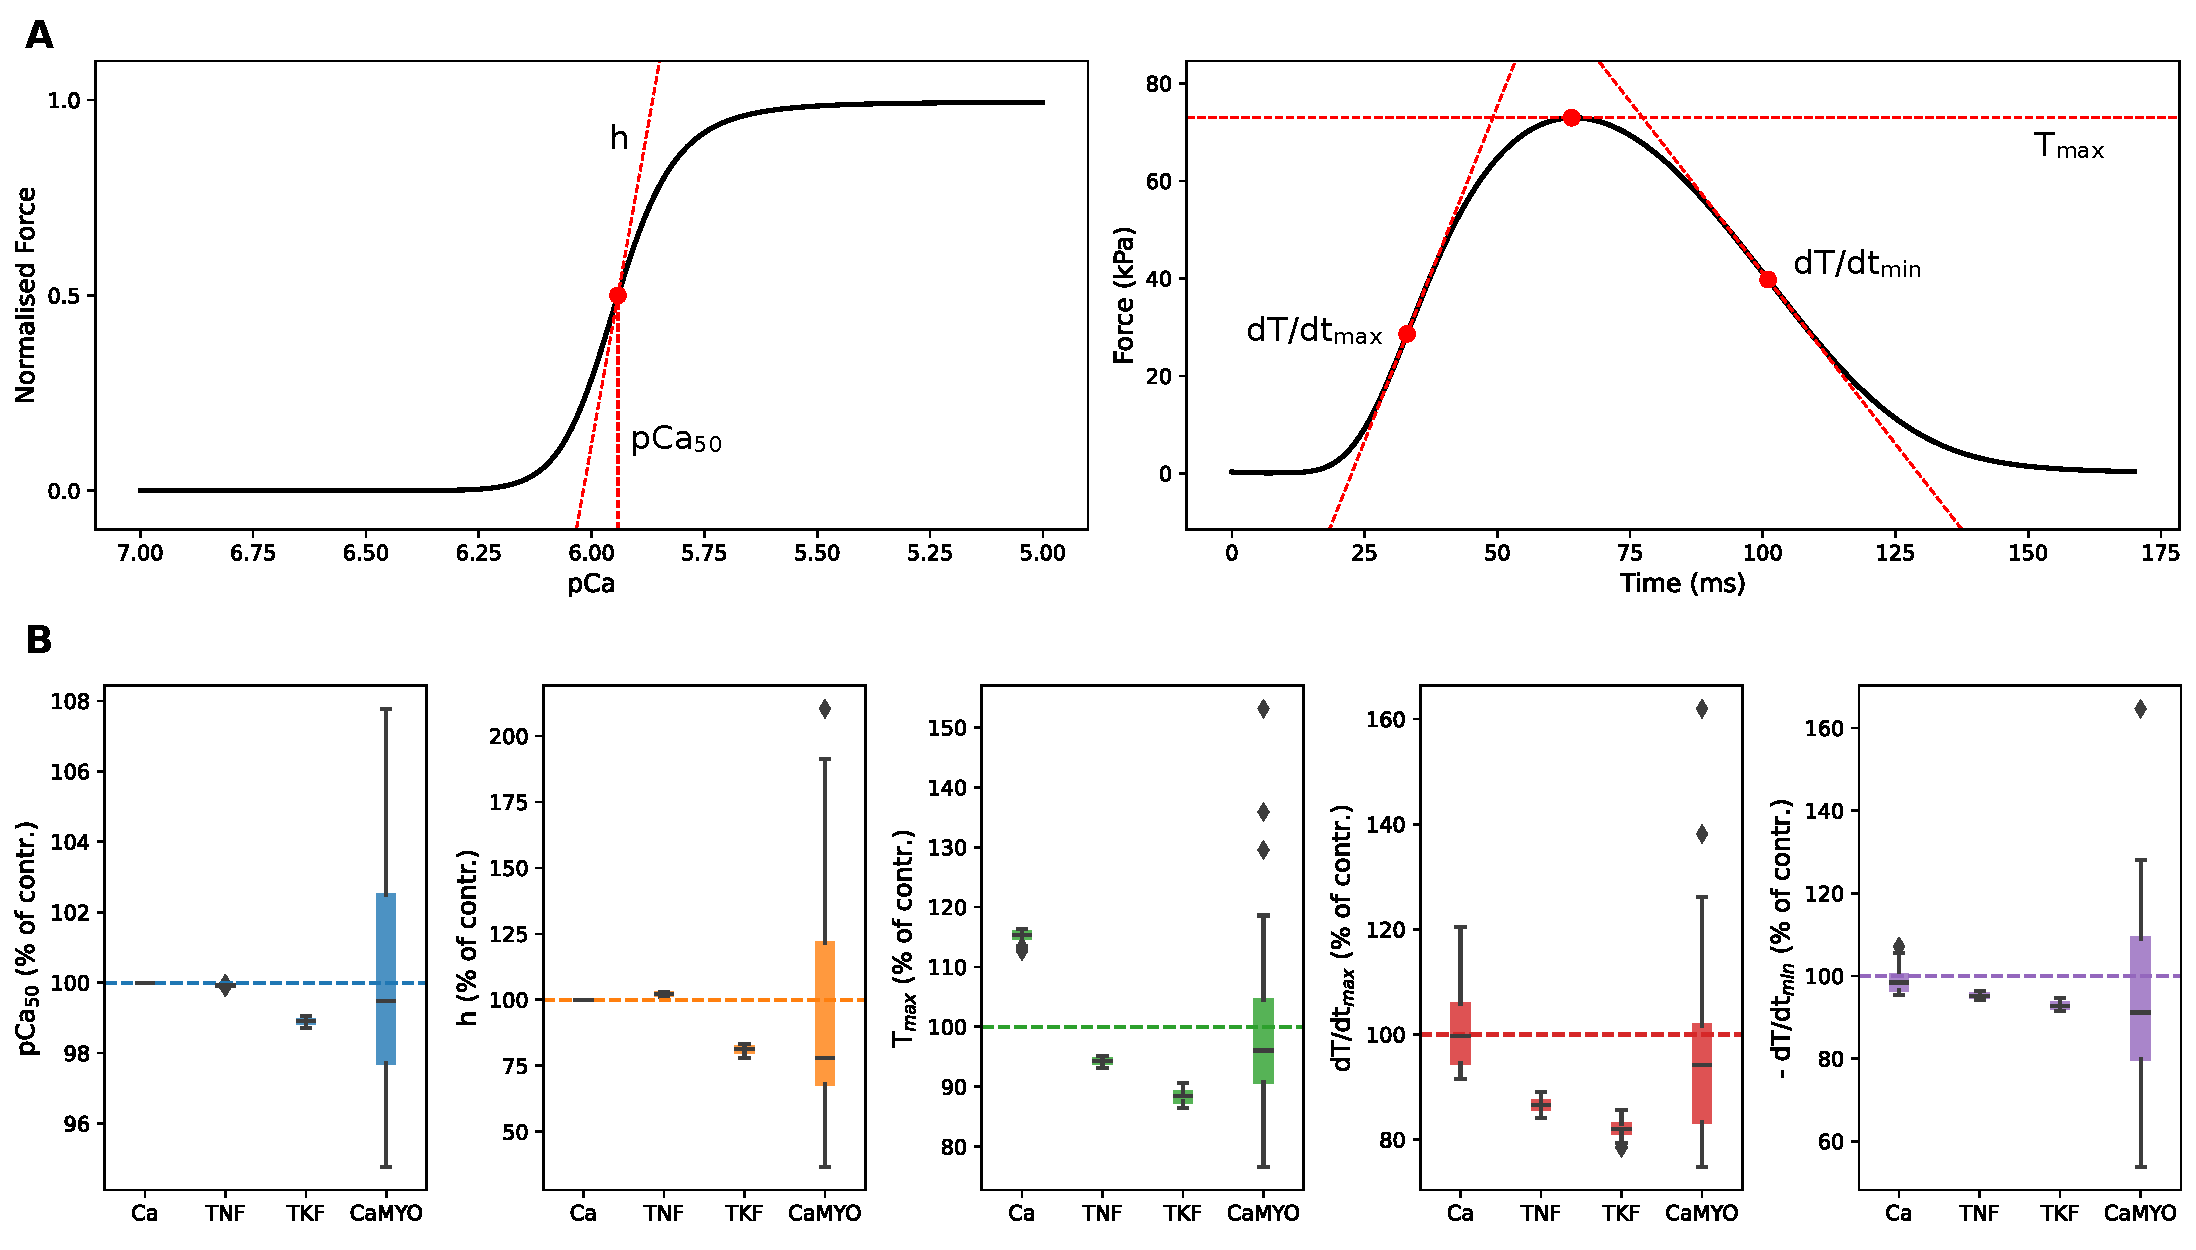
\includegraphics[width=\textwidth]{figures/chapter07/FpCa_T_trends_explained.pdf}
    \caption{Isometric force-calcium relationship and generated active tension properties from the recovered rat model parameter space. (A) Calcium sensitivity ($\pCaf$) and Hill coefficient ($h$) features are extracted from the F-pCa curve, while peak tension ($\textrm{T}_{max}$) and maximum rates of tension development ($\textrm{dT/dt}_{max}$) and decay ($\textrm{dT/dt}_{min}$) are extracted from the twitch transient. (B) Distributions of extracted $\pCaf$ (blue), $h$ (orange), $\textrm{T}_{max}$ (green), $\textrm{dT/dt}_{max}$ (red), $\textrm{dT/dt}_{min}$ (purple) values are compared with the respective ZSF1 rat model baseline values (dashed lines).}
    \label{fig:fpcatension}
\end{figure}


%
%
%
\section{Discussion}\label{sec:ch7discussion}
In this study, we proposed that $\Ca$ dynamics, thin and thick filaments kinetics are all potential pharmacological targets for HFpEF, based on simulations in the ZSF1 rat model. The found recovered rat model parameter space, when interpreted in terms of muscle experimental measurements, also suggested that HFpEF-treating compounds should possibly act as direct sarcomere modulators by desensitising the myofilament and reducing the affinity to intracellular $\Ca$, and decreasing the maximum generated active force while slowing down active force generation and relaxation in the intact muscle.

\vspace{0.2cm}
The targets identified in this study (Figure~\ref{fig:paramsdistr}) are consistent with the common end point of the two example pharmacotherapies for HFpEF treatment presented in Section~\ref{sec:ch1HF_with_preserved_ejection_fraction}. Specifically, both the Ca and the CaMYO strategies of recovery proposed a decrease (of $\sim\SI{30}{}-\SI{50}{\percent}$ from the diseased animal reference value) in the half-maximal $\Ca$ relaxation time, making less calcium available during the cardiac cycle. However, if this is accompanied by only a slight increase ($\sim\SI{5}{}-\SI{10}{\percent}$) in the diastolic $\Ca$ concentration, a very prolonged ($\sim\SI{40}{}-\SI{60}{\percent}$) time to peak $\Ca$ concentration is present as well, although this affects mostly the tension development and duration, rather then relaxation. We have seen that the Ca and CaMYO strategies have proposed a $\Ca$ transient which is slower to rise and faster to decline, corresponding to a delayed and more symmetric $\Ca$ transient. This causes a far greater delay between activation and contraction and a delayed systole, also visible in the left- and right-most panels in Figure~\ref{fig:bestfits}. However, as more time is spent in isovolumetric contraction with unaltered ejection times, this results in negligible negative effects on the cardiac output. At the same time, this is accompanied by a shorter diastole, which in the case of HFpEF pathology constitutes an improvement for cardiac relaxation.

\vspace{0.2cm}
Although $\Ca$ dynamics and sarcomere modulators are already subject of ongoing clinical trials (Section~\ref{sec:ch1HF_with_preserved_ejection_fraction}), the strategies of recovery proposed in this study by the TNF, TKF and CaMYO parameter groups cannot be directly compared to what is currently being tested experimentally, therefore they still miss thorough validation. Nevertheless, in Chapter~\ref{cha:chapter5} we have shown that single compounds' effects can be quantitatively validated using mathematical models. As previous works (e.g.~\cite{Fernandez-Chas:2018}) have demonstrated how models could be used for transferring findings between species, we don't exclude the possibility for this framework to be scaled to human scale models, in order to potentially help the designing and developing of future diagnostic and therapeutic strategies.


%
%
%
\subsection{Limitations}\label{sec:ch7limitations}
The performed GSA showed that altering preload and afterload has a secondary impact on the overall LV function. However, we modelled these two factors as fixed boundaries, and in more sophisticated closed loops heart systems the situation might change. The GSA also highlighted that parameters $\kxb$ and $\tref$ related to cross-bridge dynamics had a limited impact on haemodynamic features such as SV or EF. This may be in part due to the length dependence of tension, where decreased $\tref$ or $\kxb$ will lead to slower tension development, which will lead to the muscle remaining at higher sarcomere lengths for longer, and hence having higher $\Ca$ sensitivity, which in turn will recover contraction.

\vspace{0.2cm}
Considering the high sensitivity of EF to $\tref$ reported in other uncertainty quantification of LV cardiac function studies (e.g.~\cite{Campos:2020}), we further investigated into this apparently controversial finding by performing an additional \textit{one-at-a-time} sensitivity analysis. We selected $5$ parameters that were identified as the most important by the GSA, namely $\dca$, $\ampl$, $\Caif$, $\ntrpn$, $\trpnf$, and we further selected the $\kxb$ and $\tref$ parameters which were shown to have a limited impact instead. The SHAM rat model was then run at a fixed, reference parameter set (Table~\ref{tab:bestfitparametersvalues}) with only one parameter taking equally-spaced values in the $\pm\SI{50}{\percent}$ range of perturbation from its baseline value. The converging mechanics simulations' output PV loops were analysed to extract the corresponding EDV, ESV, SV and EF features' values, given as percentages from their baseline values (Table~\ref{tab:bestfitfeaturesvalues}). The process was repeated separately for each of the $7$ model parameters considered. In this way, each output LV feature response to each input parameter could be obtained.

\begin{figure}[ht!]
    \myfloatalign
    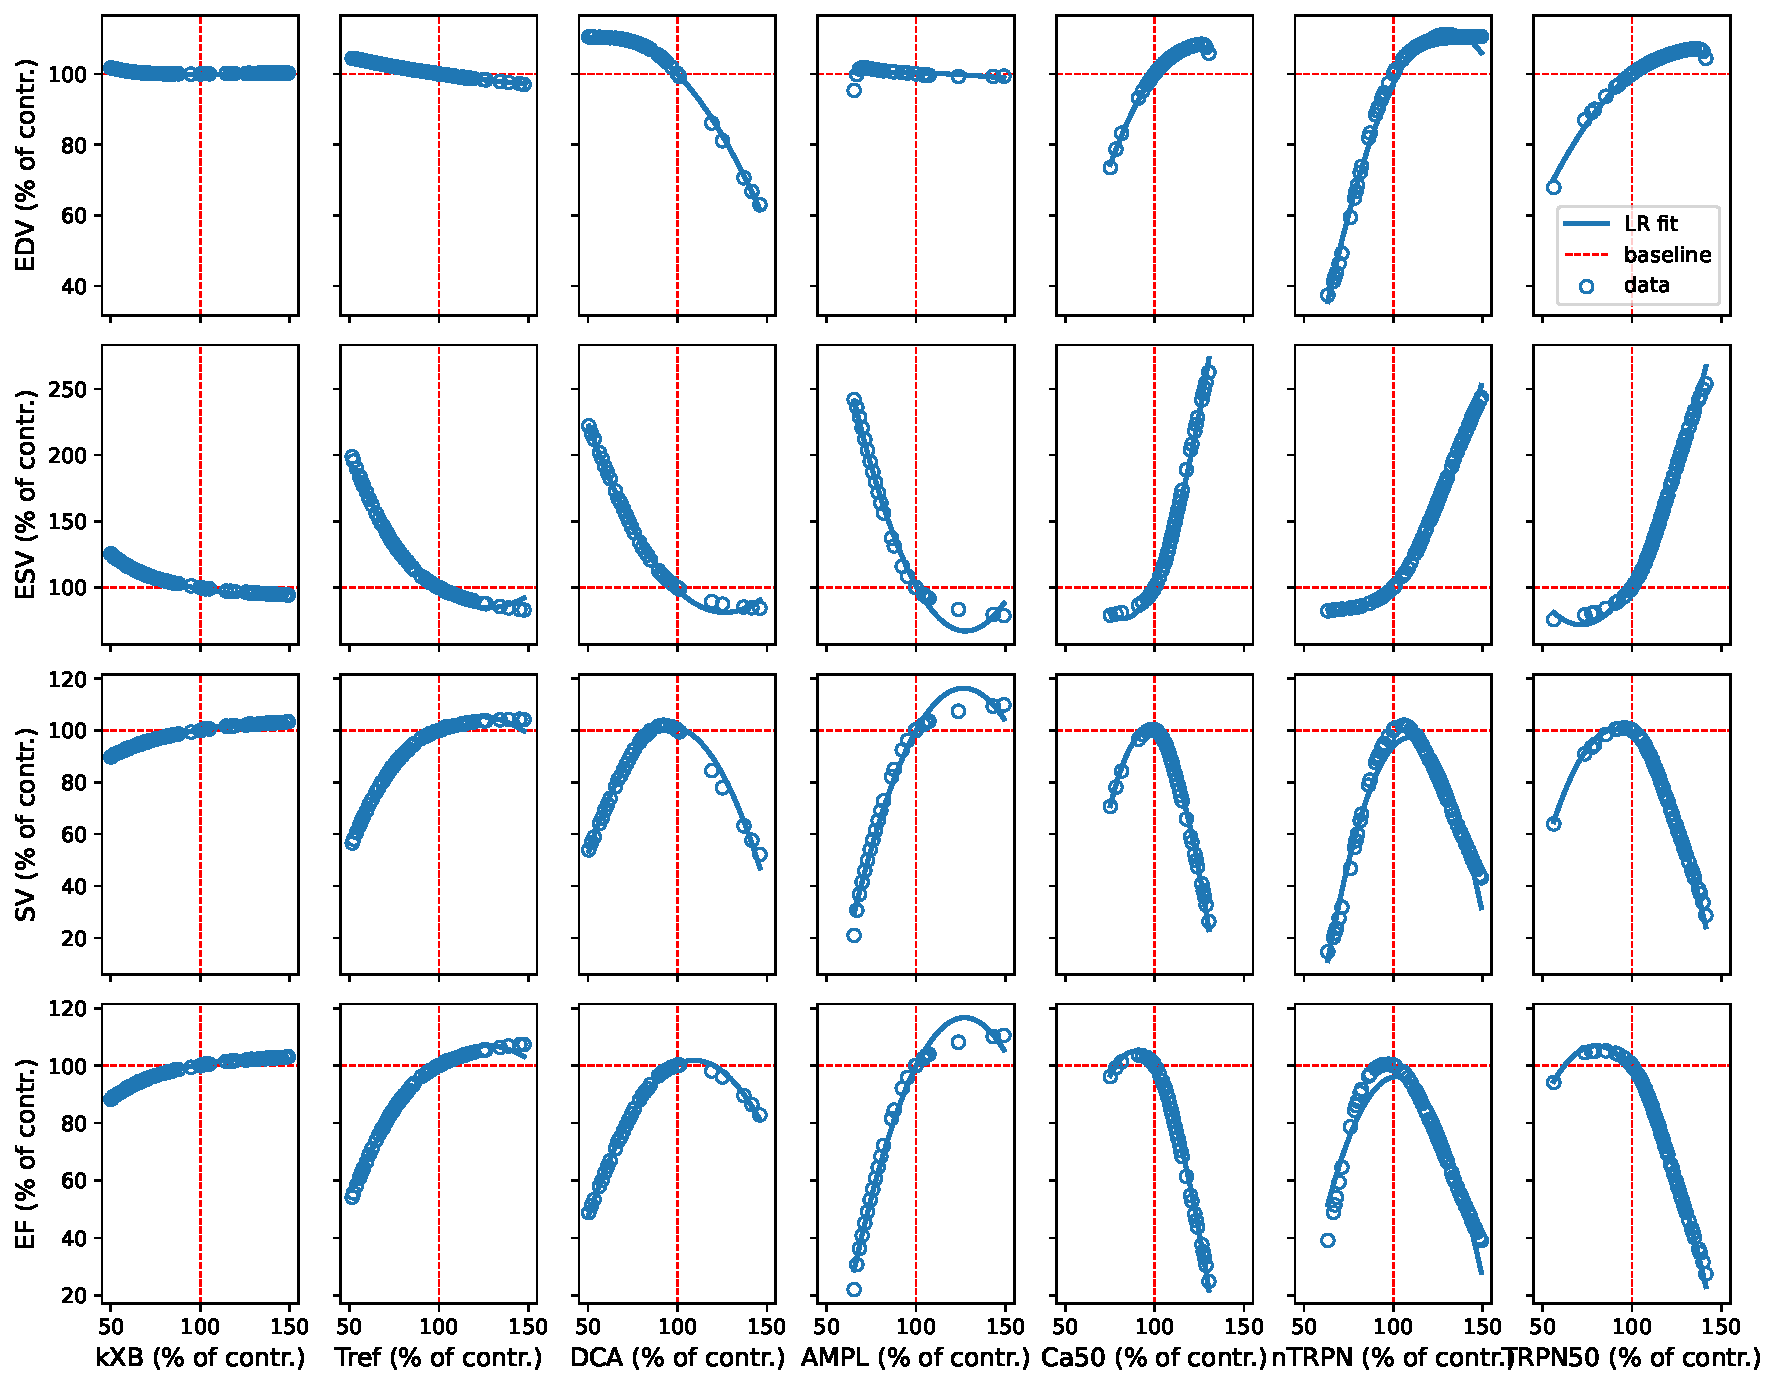
\includegraphics[width=\textwidth]{figures/chapter07/Figure_oneatatime_thesis.pdf}
    \caption{Personalised healthy rat heart contraction model LV volume features' response to model parameters' one-at-a-time variation. Both input parameters and output features are given as percentages of their baseline values (vertical and horizontal red dashed lines, respectively). Simulated features' values are displayed as open blue dots. A linear regression (LR) model with second-order degree polynomials is fitted to the data (blue lines) to facilitate visualisation of non-linear and non-monotonic relationships between the features and each of the parameters considered.}
    \label{fig:oat}
\end{figure}

\vspace{0.2cm}\noindent
Although the $\kxb$ and $\tref$ parameters resulted in a non-negligible impact on the considered LV features, we can state that the results from this sensitivity analysis are consistent with the GSA results (Section~\ref{sec:ch7model_emulators_and_output_sensitivities}). In Figure~\ref{fig:oat}, we can see that the relationship between the considered input parameters and output features is non-linear and non-monotonic. Moreover, we can see that the parameters identified as the most important by the GSA are operating at a maximum with their reference values, where a small change can cause a sharp variation in the slope of LV features' variation, whereas $\kxb$ and $\tref$ are operating on a stable slope where their impact is saturating.

\vspace{0.2cm}
In Section~\ref{sec:ch7personalised_healthy_rat_model_validation_using_emulators} we have seen that the emulators were able to predict with high accuracy the same quantitative compounds' effects on the examined LV features as the ones obtained using the simulator. However, the accuracy notably decreased and uncertainties increased when predicting high compound concentration values. We know that high concentrations of $\Ca$ channel blockers are associated with vanishing $\Ca$ transients. Since vanishing $\Ca$ transients also made the simulator fail due to small $\Ca$ signal amplitudes (Section~\ref{sec:ch7training_dataset_emulators_global_sensitivity_analysis}), the training dataset consequently did not contain parameter points encoding this kind of $\Ca$ transient shape. Therefore, predicting high compound concentration regions resulted in performing extrapolation outside the emulators' training space boundaries, which can explain the observed reduction in prediction accuracy.

\vspace{0.2cm}
Building a ZSF1 rat model by perturbing the SHAM model is a pragmatic choice. Ideally, one would want to start from MRI images of the obese ZSF1 rat and its related control (lean ZSF1 rat), create an \textit{in silico} representation of both by fitting model parameters to haemodynamic measurements (possibly obtained from the same experimental rats cohorts) and then attempt to ``virtually" recover the obese rat (diseased state) towards the lean rat (healthy state). The calculated percentages of recovery pointed out that all the parameter groups are able to recover cardiac function of similar degrees. Since every parameter group represents a strategy of recovery, this results in weighting all the types of recovery equally, and in real life situations each of them might have a different weight of clinical importance. However, this information can potentially be included in our analysis by weakening or strengthening the implausibility criterion for parameters that have to be more important than others.

\vspace{0.2cm}
More general limitations of the adopted modelling framework can be found in Chapter~\ref{cha:chapter9}, Section~\ref{sec:ch9limitations}.


%
%
%
\section{Summary}\label{sec:ch7summary}
We have used a validated biophysically detailed computational model of $3$D biventricular rat heart mechanics and a Bayesian probabilistic framework to provide indication of potential cellular pharmacological targets to evaluate recovery of the LV function in an animal model of HFpEF. This combination of forward deterministic modelling with machine learning techniques proved to be crucial to carry out analysis which are normally too computational intensive to be performed within reasonable timescales. The developed framework can easily be adapted to solve many other different systems biology problems and could potentially aid the drug discovery and development process at preclinical stages.
% \vspace{0.2cm}
% We developed a computational model of the ZSF1 rat model of heart failure with preserved ejection fraction. We validated that the model can link simulated pharmacological interventions from cellular to whole heart pump function. Our computational model identified $\Ca$ dynamics as the main determinant of left ventricular contractile behaviour. We demonstrated that the highest degree of LV function recovery could be achieved when $\Ca$ dynamics is manipulated in conjunction with both thin and thick filament kinetics.